\chapter{GPU Convolution}
\label{chap:gpu_convolution}
Convolution is one of the most important tools in any digital signal processing engineer’s toolbox. 
Convolution can be implemented in the time or frequency domain. 
%In CPUs, the number of floating point operations (flop) is the main determining factor in execution time.
%The Tesla K40c can perform 4.29 Tflops, computation is not a problem.
%The limiting factor in GPUs is the memory bandwidth.
Theory says if the given filter is ``long'', the frequency domain is the best choice.
But how long is… long? 
First we need a way to measure how computationally intensive an algorithm is. 
The number of flops is commonly used for benchmarking. 
Let the complex signal length be $N$ and the complex filter length be $L$.
Each complex multiply 
\begin{equation}
(A+jB)\times(C+jD) = (AC-BD)+j(AD+BC)
\end{equation}
is $6$ flops, $4$ multiplies and $2$ additions/subtractions.

Discrete time convolution computed in the time domain is
\begin{equation}
y(n) = \sum^{L-1}_{m=0} x(m) h(n-m).
  \label{eq:simple_conv_time}
\end{equation}
Each output element of $y(n)$ requires a $8L$ flops, $2$ flops (real and imaginary) for each term to be summed then $6$ flops for time signal and filter complex multiply.
The length of the output $\mathbf{y}$ is $N+L-1$.
The number of flops required for convolution of a given length $N$ signal and length $L$ filter is
\begin{equation}
8L(N+L-1) \text{ flops}.
\label{eq:flops_time_domain_conv}
\end{equation}

Discrete time convolution computed in the frequency domain is
\begin{equation}
\mathbf{y} = \mathscr{F}^{-1}(\mathscr{F}(\mathbf{x})\times\mathscr{F}(\mathbf{h})).
  \label{eq:simple_conv_freq}
\end{equation}
The length of the convolution, $M=N+L-1$ is the minimum point Fourier Transform possible.
It is common practice perform a next power of two above the minimum Fourier Transform to leverage the Cooley-Tukey radix 2 Fast Fourier Transform (FFT).
In the Fastest Fourier Transform in the West (FFTW) library the Cooley-Tukey radix 2 transform is used.
Each radix 2 forward or backward Fourier transform performs $5M\log_2(M)$ flops \cite{FFTW:2017,cooley1965algorithm}.
Performing convolution in the frequency domain requires
\begin{equation}
3\times5M\log_2(M)+6M \text{ flops}.
\label{eq:flops_freq_domain_conv}
\end{equation}

\section{Single Convolution}
\label{sec:cuda_convolution_single}
Figure \ref{fig:Theory186Tap_flops} compares the number of flops required for time domain verse frequency domain convolution of a $12672$ sample complex signal with a $186$ tap complex filter.
Figure \ref{fig:Theory21Tap_flops} compares the number of flops required for time domain verse frequency domain convolution of a $12672$ sample complex signal with a $21$ tap complex filter.
Appending zeros to the next power of $2$ causes the stair stepping pattern.
\begin{figure}
	\caption{Comparison of number of floating point operations (flops) required to convolve a $12672$ sample complex signal with a $186$ tap complex filter.}
	\centering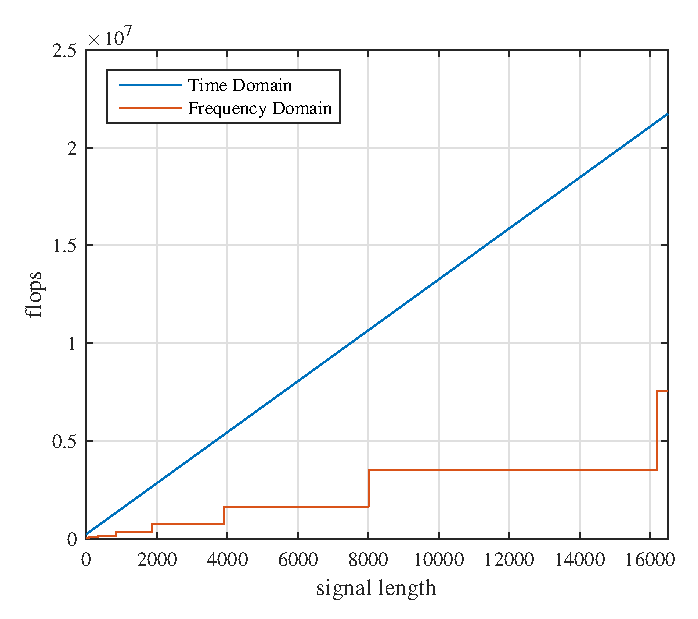
\includegraphics[width=5in]{figures/gpu_intro/Theory186Tap_flops.eps}
	\label{fig:Theory186Tap_flops}
\end{figure}
\begin{figure}
	\caption{Comparison of number of floating point operations (flops) required to convolve a $12672$ sample complex signal with a $21$ tap complex filter.}
	\centering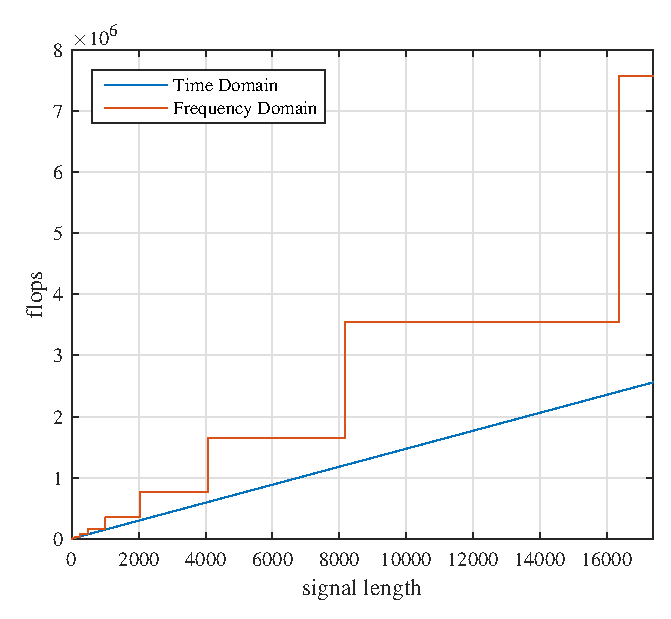
\includegraphics[width=5in]{figures/gpu_intro/Theory21Tap_flops.eps}
	\label{fig:Theory21Tap_flops}
\end{figure}


Now that we understand the number of flops required for a ``short'' filter, does the number of flops affect CPU or GPU execution time?
While Listing \ref{code:GPUvsCPU} is a simple and good example showing how program GPUs, frankly, it is pretty boring and doesn't display the real challenges and tradeoffs of GPUs.
Listing \ref{code:convFun} shows five different ways of implementing convolution:
\begin{itemize}
  \item time domain convolution in a CPU
  \item frequency domain convolution in a CPU
  \item time domain convolution in a GPU using global memory
  \item time domain convolution in a GPU using shared memory
  \item frequency domain convolution in a GPU using CUDA libraries
\end{itemize}
The CPU implements Equation \eqref{eq:simple_conv_time} in ConvCPU directly on line $209$ using a function from lines $11$ to $34$.
The CPU implements Equation \eqref{eq:simple_conv_freq} using the FFTW library on lines $214$ to $258$.
The GPU implements time domain convolution using global memory in lines $268$ to $277$.
The GPU kernel ConvGPU on lines $36$ to $64$ is a parallel version of ConvCPU.
ConvGPU implements time domain convolution by accessing global memory for every element of the signal and filter.
The GPU implements time domain convolution using shared memory in lines $283$ to $292$.
The GPU kernel ConvGPUshared on lines $67$ to $101$ is nearly identical to ConvGPU.
Threads accessing the same elements of the filter in global memory is a waste of valuable clock cycles.
ConvGPUshared pays and initial price on lines $72$ to $76$ to move $L_\text{h}$ filter coefficients from off chip global memory memory to on chip shared memory.
Finally, the GPU implements frequency domain convolution using the cuFFT library on lines $298$ to $326$.


So the questions are:
Do flops have a direct relationship to execution time on CPUs? 
Do flops have a direct relationship to execution time on GPUs? 
When is convolution in CPUs faster than GPUs?
When is it worth the initial cost to used shared memory?
When should convolution be done in the frequency domain?

The answer to all of the questions is...it depends on your signal length, filter length, CPU, GPU and memory.
A CUDA programmer can make an educated guess on which algorithm may be faster, but until all the algorithms have been implemented and timed, there is no definite answer.

To demonstrate that there is no definite answer in GPUs, 
the execution time of the code in Listing \ref{code:GPUvsCPU} was timed.
Only the CPU functions were timed for the time and frequency domain convolution on the CPU.
Each memory transfer host to device and device to host was timed for a fair comparison of GPU to CPU.
Table \ref{tab:CPUvsGPUtimingTable} shows where timing was started and stopped for each algorithm.
\begin{table}
\caption{Defining start and stop lines for timing comparison in Listing \ref{code:convFun}.}
\begin{center}
\begin{tabular}{llll}
	\toprule
	Algorithm 				& Function		& Start Line	& Stop  Line		\\ \midrule
	CPU time domain 		& ConvCPU 		& 208			& 210 				\\
	CPU frequency domain 	& FFTW 			& 213			& 259 				\\
	GPU time domain global 	& ConvGPU 		& 267			& 278				\\
	GPU time domain shared 	& ConvGPUshared & 282			& 293				\\
	GPU frequency domain 	& cuFFT			& 301			& 327				\\ 
	\bottomrule
\end{tabular}
\end{center}
\label{tab:CPUvsGPUtimingTable}
\end{table}

Figure \ref{fig:CPUvsGPU_1batch_186taps_varySignal_noMin} compares the computation time of a fixed length $186$ tap filter convolved with a varied length signal.
The execution time varies enough that the plot is messy and unreadable.
Figure \ref{fig:CPUvsGPU_1batch_186taps_varySignal} compares the same data but $15$ sample local minimums were found.
\begin{figure}
	\caption{Comparison of a complex convolution on CPU verse GPU. The signal length is varied and the filter is fixed at $186$ taps. The comparison is messy with out lower bounding.}
	\centering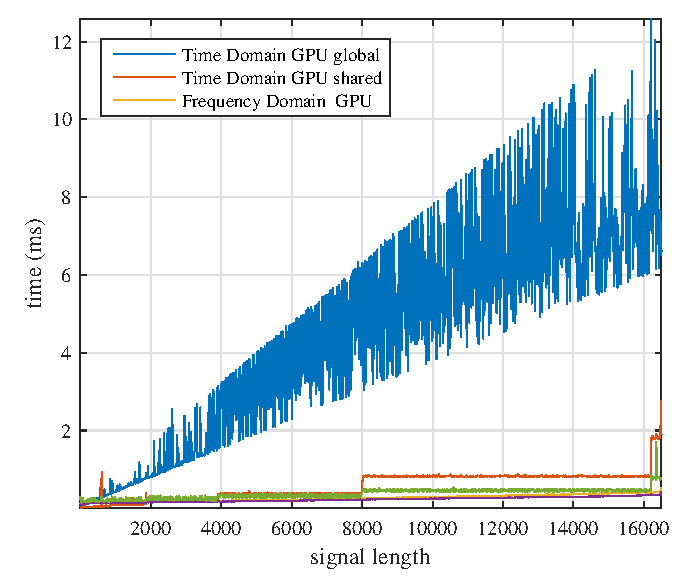
\includegraphics[width=5in]{figures/gpu_intro/CPUvsGPU_1batch_186taps_varySignal_noMin.eps}
	\label{fig:CPUvsGPU_1batch_186taps_varySignal_noMin}
\end{figure}
\begin{figure}
	\caption{Comparison of a complex convolution on CPU verse GPU. The signal length is varied and the filter is fixed at $186$ taps. A lower bound was applied by searching for a local minimums in $15$ sample width windows.}
	\centering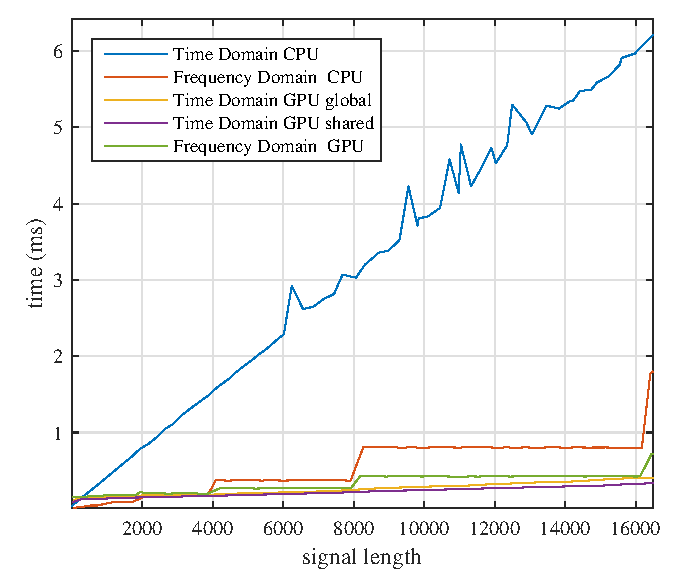
\includegraphics[width=5in]{figures/gpu_intro/CPUvsGPU_1batch_186taps_varySignal.eps}
	\label{fig:CPUvsGPU_1batch_186taps_varySignal}
\end{figure}

With the plot lower bounded, compare Figure \ref{fig:CPUvsGPU_1batch_186taps_varySignal} to Figure \ref{fig:Theory186Tap_flops}.
Does the CPU and GPU follow the same trend as the number of flops?
The CPU has the exact structure that the number of flops predicted.
The GPU does have the stair stepping from appending zeros for the frequency domain, but the time domain GPU kernels execute in less time.

The GPU execution time does not follow the same trend as the number of flops.
Why? As mentioned in Section \ref{sec:GPU_memory}, GPUs have a hanes amount of computational resources and limited memory bandwidth.
Over $90\%$ of GPU kernels are memory bandwidth limited.

To provide more proof, compare Figures \ref{fig:CPUvsGPU_1batch_21taps_varySignal} and \ref{fig:Theory21Tap_flops}.
Once again, the CPU follows the same trend as the number of flops.
The GPU also follows the number of flops trends but to a lesser extent than the CPU.
On ``short'' filters, using shared memory will perform better than using only global memory.
Using shared memory to store the short filter saves the each iteration a lot of execution time.
\begin{figure}
	\caption{Comparison of a complex convolution on CPU verse GPU. The signal length is varied and the filter is fixed at $21$ taps. A lower bound was applied by searching for a local minimums in $5$ sample width windows.}
	\centering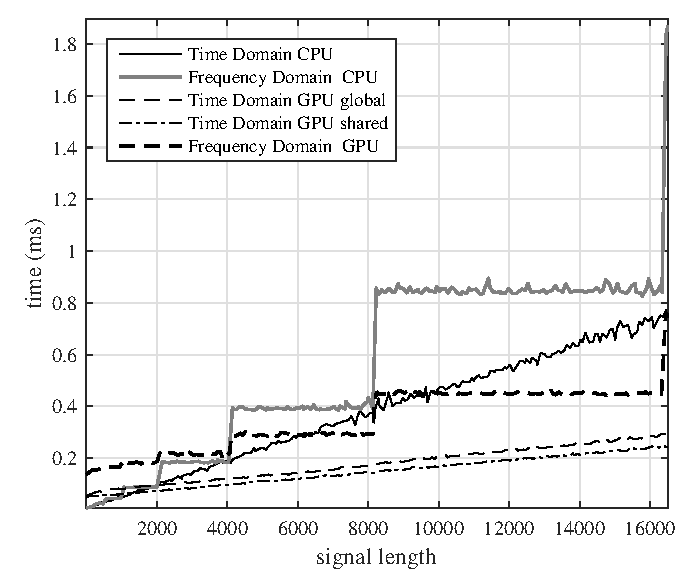
\includegraphics[width=5in]{figures/gpu_intro/CPUvsGPU_1batch_21taps_varySignal.eps}
	\label{fig:CPUvsGPU_1batch_21taps_varySignal}
\end{figure}

What if the signal length was set and the filter length was varied?
Figure \ref{fig:CPUvsGPU_1batch_12672signal_varyFilter} compares CPU to GPU execution time of a $12672$ sample signal convolved with a varying filter length.
The time domain CPU execution time is affected obviously because the number of flops increases.

Neither CPU or GPU frequency domain execution time is affected by varying filter length.
The execution time stays the same because the number of memory accesses and flops remain constant because the filter is appended with zeros to the convolution length.

The execution time of both time domain GPU convolutions are slightly affected by increasing filter length.
The number of memory accesses per output sample increase as the filter length increases.
Bottom line, the length of the signal is the largest factor as Equations \ref{eq:flops_time_domain_conv} and \ref{eq:flops_freq_domain_conv} suggest.
\begin{figure}
	\caption{Comparison of a complex convolution on CPU verse GPU. The filter length is varied and the signal is fixed at $12672$ samples. A lower bound was applied by searching for a local minimums in $3$ sample width windows.}
	\centering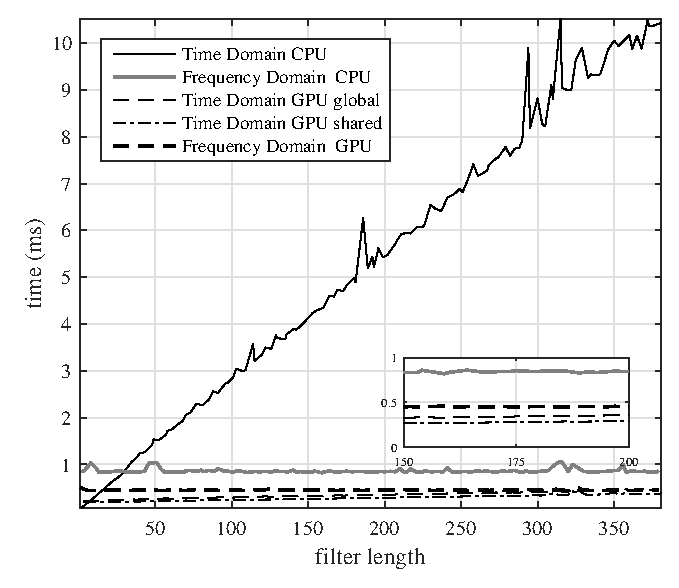
\includegraphics[width=5in]{figures/gpu_intro/CPUvsGPU_1batch_12672signal_varyFilter.eps}
	\label{fig:CPUvsGPU_1batch_12672signal_varyFilter}
\end{figure}

Conclusion, when needing implement convolution in a CPU or GPU, implement it every way possible.
Which ever way has the fastest execution time, he is your winner.
Long story short, most of the time a GPU DSP engineer is given a set length for the signal and filter.
As Figures \ref{fig:CPUvsGPU_1batch_186taps_varySignal_noMin} through \ref{fig:CPUvsGPU_1batch_12672signal_varyFilter} have shown, unless every implementation is explored, there is no way of saying which implementation will absolutely be fastest.

Table \ref{tab:CPUvsGPUtable_12672_186} shows GPU frequency domain is fastest when convolving a $12672$ sample signal with a $186$ tap filter.
Table \ref{tab:CPUvsGPUtable_12672_21} shows GPU time domain using shared is fastest when convolving a $12672$ sample signal with a $21$ tap filter.
\begin{table}
\caption{Convolution computation times with signal length $12672$ and filter length $186$ on a Tesla K40c GPU.}
\begin{center}
\begin{tabular}{lll}
	\toprule
	Algorithm 				& Function or Library		& Execution Time (ms) \\ \midrule
	CPU time domain 		& ConvCPU 					& 5.0388		\\
	CPU frequency domain 	& FFTW 						& 1.6295		\\
	GPU time domain global 	& ConvGPU 					& 0.4021		\\
	GPU time domain shared 	& ConvGPUshared 			& 0.3752		\\
	GPU frequency domain 	& cuFFT						& 0.3387		\\ 
	\bottomrule
\end{tabular}
\end{center}
\label{tab:CPUvsGPUtable_12672_186}
\end{table}
\begin{table}
\caption{Convolution computation times with signal length $12672$ and filter length $21$ on a Tesla K40c GPU.}
\begin{center}
\begin{tabular}{lll}
	\toprule
	Algorithm 				& Function or Library		& Execution Time (ms) \\ \midrule
	CPU time domain 		& ConvCPU 					& 0.6125		\\
	CPU frequency domain 	& FFTW 						& 2.5947		\\
	GPU time domain global 	& ConvGPU 					& 0.2405		\\
	GPU time domain shared 	& ConvGPUshared 			& 0.2112		\\
	GPU frequency domain 	& cuFFT						& 0.3360		\\ 
	\bottomrule
\end{tabular}
\end{center}
\label{tab:CPUvsGPUtable_12672_21}
\end{table}

\section{Batched Convolution}
In section \ref{sec:cuda_convolution_single} convolution of a single single with a single filter was studied.
Chapter blah (system overview) shows the packetized structure of the received signal.
The received signal has $3104$ packets or batches and each packet is independent of other packets.

Now that we have $3104$ signals to be convolved with $3104$ filters, how does the problem change?
Which approach to convolution will be fastest?

As the number of batches increases, does CPU and GPU execution time increase linearly?
Figure \ref{fig:CPUvsGPU_varyBatches_186taps_12672signal} shows how the execution time increases with the number of batches.
Note that no lower bounding is needed to produce clean batched processing results.
This figure shows that frequency domain convolution leverages batch processing better than time domain convolution.
No surprise CPU time and frequency domain execution time skyrockets as the number of batches increases.
The GPU handles batched processing very well because it introduces more parallelism.
\begin{figure}
	\caption{Comparison of a batched complex convolution on a CPU and GPU. The number of batches is varied while the signal and filter length is set to $12672$ and $186$.}
	\centering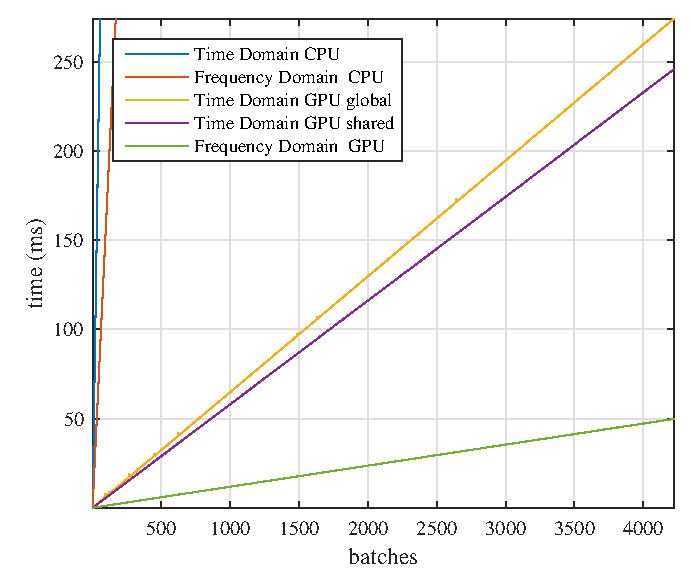
\includegraphics[width=5in]{figures/gpu_intro/CPUvsGPU_varyBatches_186taps_12672signal.eps}
	\label{fig:CPUvsGPU_varyBatches_186taps_12672signal}
\end{figure}

Judging by Figure \ref{fig:CPUvsGPU_varyBatches_186taps_12672signal}, CPU is not a contender in batched processing for fast execution times when compared to the GPU.
CPU and GPU batched processing will not be compared any further.
Listing \ref{code:batchedConvFun} shows three ways of batched convolution in CUDA
\begin{itemize}
  \item time domain convolution in a GPU using global memory
  \item time domain convolution in a GPU using shared memory
  \item frequency domain convolution in a GPU using the cuFFT library.
\end{itemize}

Now that the GPU execution time isn't being compared to the CPU, transfers between host and device will not be a factor for algorithm comparison.
Table \ref{tab:BatchedGPUtimingTable} shows how Listing \ref{code:batchedConvFun} is timed.
\begin{table}
\caption{Defining start and stop lines for timing comparison in Listing \ref{code:batchedConvFun}.}
\begin{center}
\begin{tabular}{llll}
	\toprule
	Algorithm 				& Function		& Start Line	& Stop  Line		\\ \midrule
	GPU time domain global 	& ConvGPU 		& 197			& 204				\\
	GPU time domain shared 	& ConvGPUshared & 212			& 219				\\
	GPU frequency domain 	& cuFFT			& 227			& 245				\\ 
	\bottomrule
\end{tabular}
\end{center}
\label{tab:BatchedGPUtimingTable}
\end{table}


Figure \ref{fig:CPUvsGPU_3104batch_186taps_varySignal} shows execution time for $3104$ batches of $186$ tap filters convolved with varying signal lengths.
Performing frequency domain convolution is always faster than time domain convolution because the cuFFT library is better optimized for batched processing.
Frequency domain convolution for a $12672$ sample signal takes just $36.8$ms, that is on average $0.0119$ms per batch.
Compare $0.0119$ms per batch to single batched execution time in Table \ref{tab:CPUvsGPUtable_12672_186}, one batch took $0.3387$.
Batched processing introduced a $28\times$ speed up!
\begin{figure}
	\caption{Comparison of a batched complex convolution on a GPU. The signal length is varied and the filter is fixed at $186$ taps.}
	\centering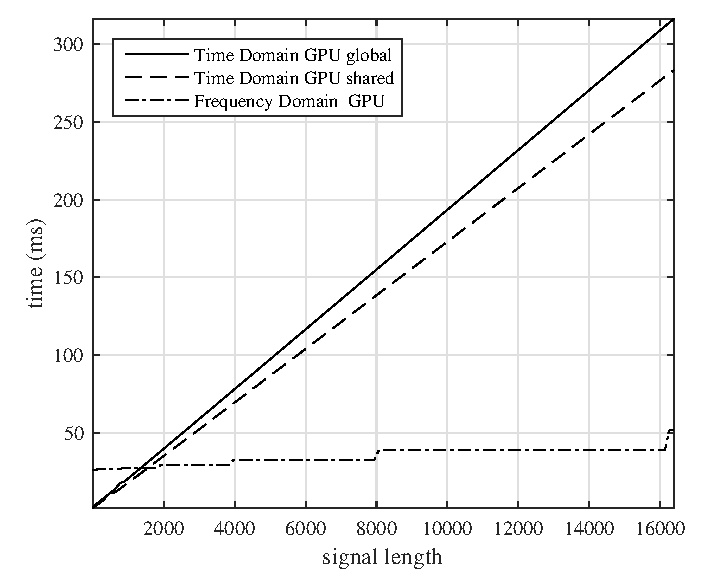
\includegraphics[width=5in]{figures/gpu_intro/CPUvsGPU_3104batch_186taps_varySignal.eps}
	\label{fig:CPUvsGPU_3104batch_186taps_varySignal}
\end{figure}

Figure \ref{fig:CPUvsGPU_3104batch_21taps_varySignal} shows execution time for $3104$ batches of $21$ tap filters convolved with varying signal lengths.
This figure exhibits the same characteristics of single batch convolution execution time shown in Figure \ref{fig:CPUvsGPU_1batch_21taps_varySignal}.
For most signal lengths, performing time domain convolution using shared memory is fastest.
\begin{figure}
	\caption{Comparison of a batched complex convolution on a GPU. The signal length is varied and the filter is fixed at $21$ taps.}
	\centering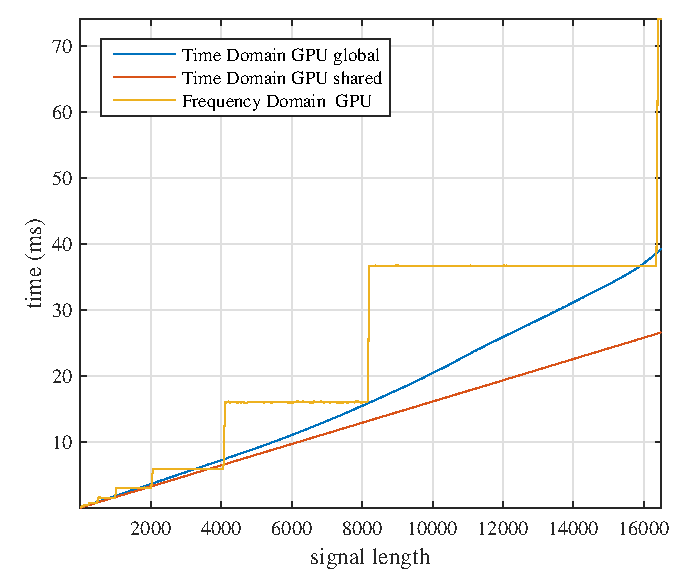
\includegraphics[width=5in]{figures/gpu_intro/CPUvsGPU_3104batch_21taps_varySignal.eps}
	\label{fig:CPUvsGPU_3104batch_21taps_varySignal}
\end{figure}

Figure \ref{fig:CPUvsGPU_3104batch_12672signal_varyFilter} shows execution time for $3104$ batches of $12672$ sample signal convolved with varying filter lengths.
This figure exhibits nearly the same characteristics of single batch convolution execution time shown in Figure \ref{fig:CPUvsGPU_1batch_12672signal_varyFilter} accept the varied filter length has no affect on execution time.
For very short filter lengths, time domain convolution using shared memory is fastest.
For longer filters , frequency domain convolution is fastest.
\begin{figure}
	\caption{Comparison of a batched complex convolution on a GPU. The signal length is varied and the filter is fixed at $21$ taps.}
	\centering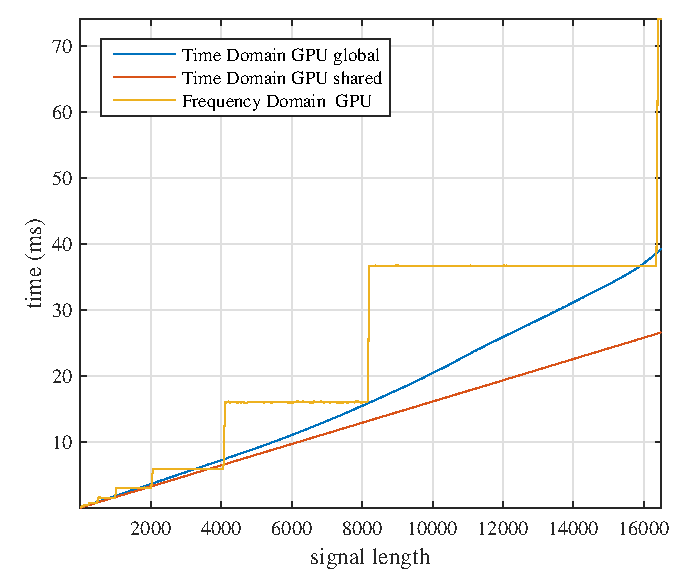
\includegraphics[width=5in]{figures/gpu_intro/CPUvsGPU_3104batch_21taps_varySignal.eps}
	\label{fig:CPUvsGPU_3104batch_21taps_varySignal}
\end{figure}

Though this section has show that in batched processing the algorithm leading to the fastest execution time still depends on signal and filter length,
one important comcept has been over looked.
Figure \ref{fig:ProcessingBlock} shows there are two filters that need to be allied to the signal. 

If convolution is implemented in the time domain, ConvGPU or ConvGPUshared must run twice.
The first call of ConvGPU or ConvGPUshared performs the convolution of the $186$ tap equalizer and $21$ detection filter.
The second call of ConvGPU or ConvGPUshared performs the convolution of the $12672$ sample signal with the  convolved $186+21-1$ tap filter.

If convolution is implemented in the frequency domain, only the GPU kernel PointToPointMultiply has to be updated.
PointToPointMultiply must be changed from two input vectors to three input vectors.
For every point the number of memory accesses increases by $1$ element and the number of flops doubles from $6$ to $12$.
An extra cuFFT call would be expected accept the detection filter in Figure \ref{fig:ProcessingBlock} constant.
The FFT of the detection filter can be calculated and stored at initialization.

Table \ref{tab:Batched_CPUvsGPUtable_12672_186} shows the batched convolution execution time for a $12672$ sample signal and $186$ tap filter.
Table \ref{tab:Batched_CPUvsGPUtable_12672_21} shows the batched convolution execution time for a $12672$ sample signal and $21$ tap filter.
Table \ref{tab:Batched_CPUvsGPUtable_12672_21_186} shows the batched cascaded convolution execution time for a $12672$ sample signal with $21$ and $186$ tap filters.
\begin{table}
\caption{Batched convolution execution times with for a $12672$ sample signal and $186$ tap filter on a Tesla K40c GPU.}
\begin{center}
\begin{tabular}{lll}
	\toprule
	Algorithm 				& Function or Library		& Execution Time (ms) \\ \midrule
	GPU time domain global 	& ConvGPU 					& 201.29		\\
	GPU time domain shared 	& ConvGPUshared 			& 180.272		\\
	GPU frequency domain 	& cuFFT						& 36.798 		\\ 
	\bottomrule
\end{tabular}
\end{center}
\label{tab:Batched_CPUvsGPUtable_12672_186}
\end{table}
\begin{table}
\caption{Batched convolution execution times with for a $12672$ sample signal and $21$ tap filter on a Tesla K40c GPU.}
\begin{center}
\begin{tabular}{lll}
	\toprule
	Algorithm 				& Function or Library		& Execution Time (ms) \\ \midrule
	GPU time domain global 	& ConvGPU 					& 27.642		\\
	GPU time domain shared 	& ConvGPUshared 			& 20.4287		\\
	GPU frequency domain 	& cuFFT						& 36.7604		\\ 
	\bottomrule
\end{tabular}
\end{center}
\label{tab:Batched_CPUvsGPUtable_12672_21}
\end{table}
\begin{table}
\caption{Batched convolution execution times with for a $12672$ sample signal and $206$ tap filter on a Tesla K40c GPU.}
\begin{center}
\begin{tabular}{lll}
	\toprule
	Algorithm 				& Function or Library		& Execution Time (ms) \\ \midrule
	GPU time domain global 	& ConvGPU 					& 223.064		\\
	GPU time domain shared 	& ConvGPUshared 			& 199.844		\\
	GPU frequency domain 	& cuFFT						& 36.7704		\\ 
	\bottomrule
\end{tabular}
\end{center}
\label{tab:Batched_CPUvsGPUtable_12672_206}
\end{table}
\begin{table}
\caption{Batched convolution execution times with for a $12672$ sample signal and cascaded $21$ and $186$ tap filter on a Tesla K40c GPU.}
\begin{center}
\begin{tabular}{lll}
	\toprule
	Algorithm 				& Function or Library		& Execution Time (ms) \\ \midrule
	GPU time domain global 	& ConvGPU 					& 223.307		\\
	GPU time domain shared 	& ConvGPUshared 			& 200.018		\\
	GPU frequency domain 	& cuFFT						& 39.0769		\\ 
	\bottomrule
\end{tabular}
\end{center}
\label{tab:Batched_CPUvsGPUtable_12672_21_186}
\end{table}

Tables \ref{tab:Batched_CPUvsGPUtable_12672_186} and \ref{tab:Batched_CPUvsGPUtable_12672_21} agree with Figures \ref{fig:CPUvsGPU_3104batch_21taps_varySignal} and \ref{fig:CPUvsGPU_3104batch_186taps_varySignal}.
Time domain convolution is faster with a short $21$ tap filter but frequency domain convolution is faster with a long $186$ tap filter.

\begin{figure}
	\caption{Two ways to convolve the signal $\mathbf{r}$ with the $186$ tap filter $\mathbf{c}$ and $21$ tap filter $\mathbf{d}$.}
	\centering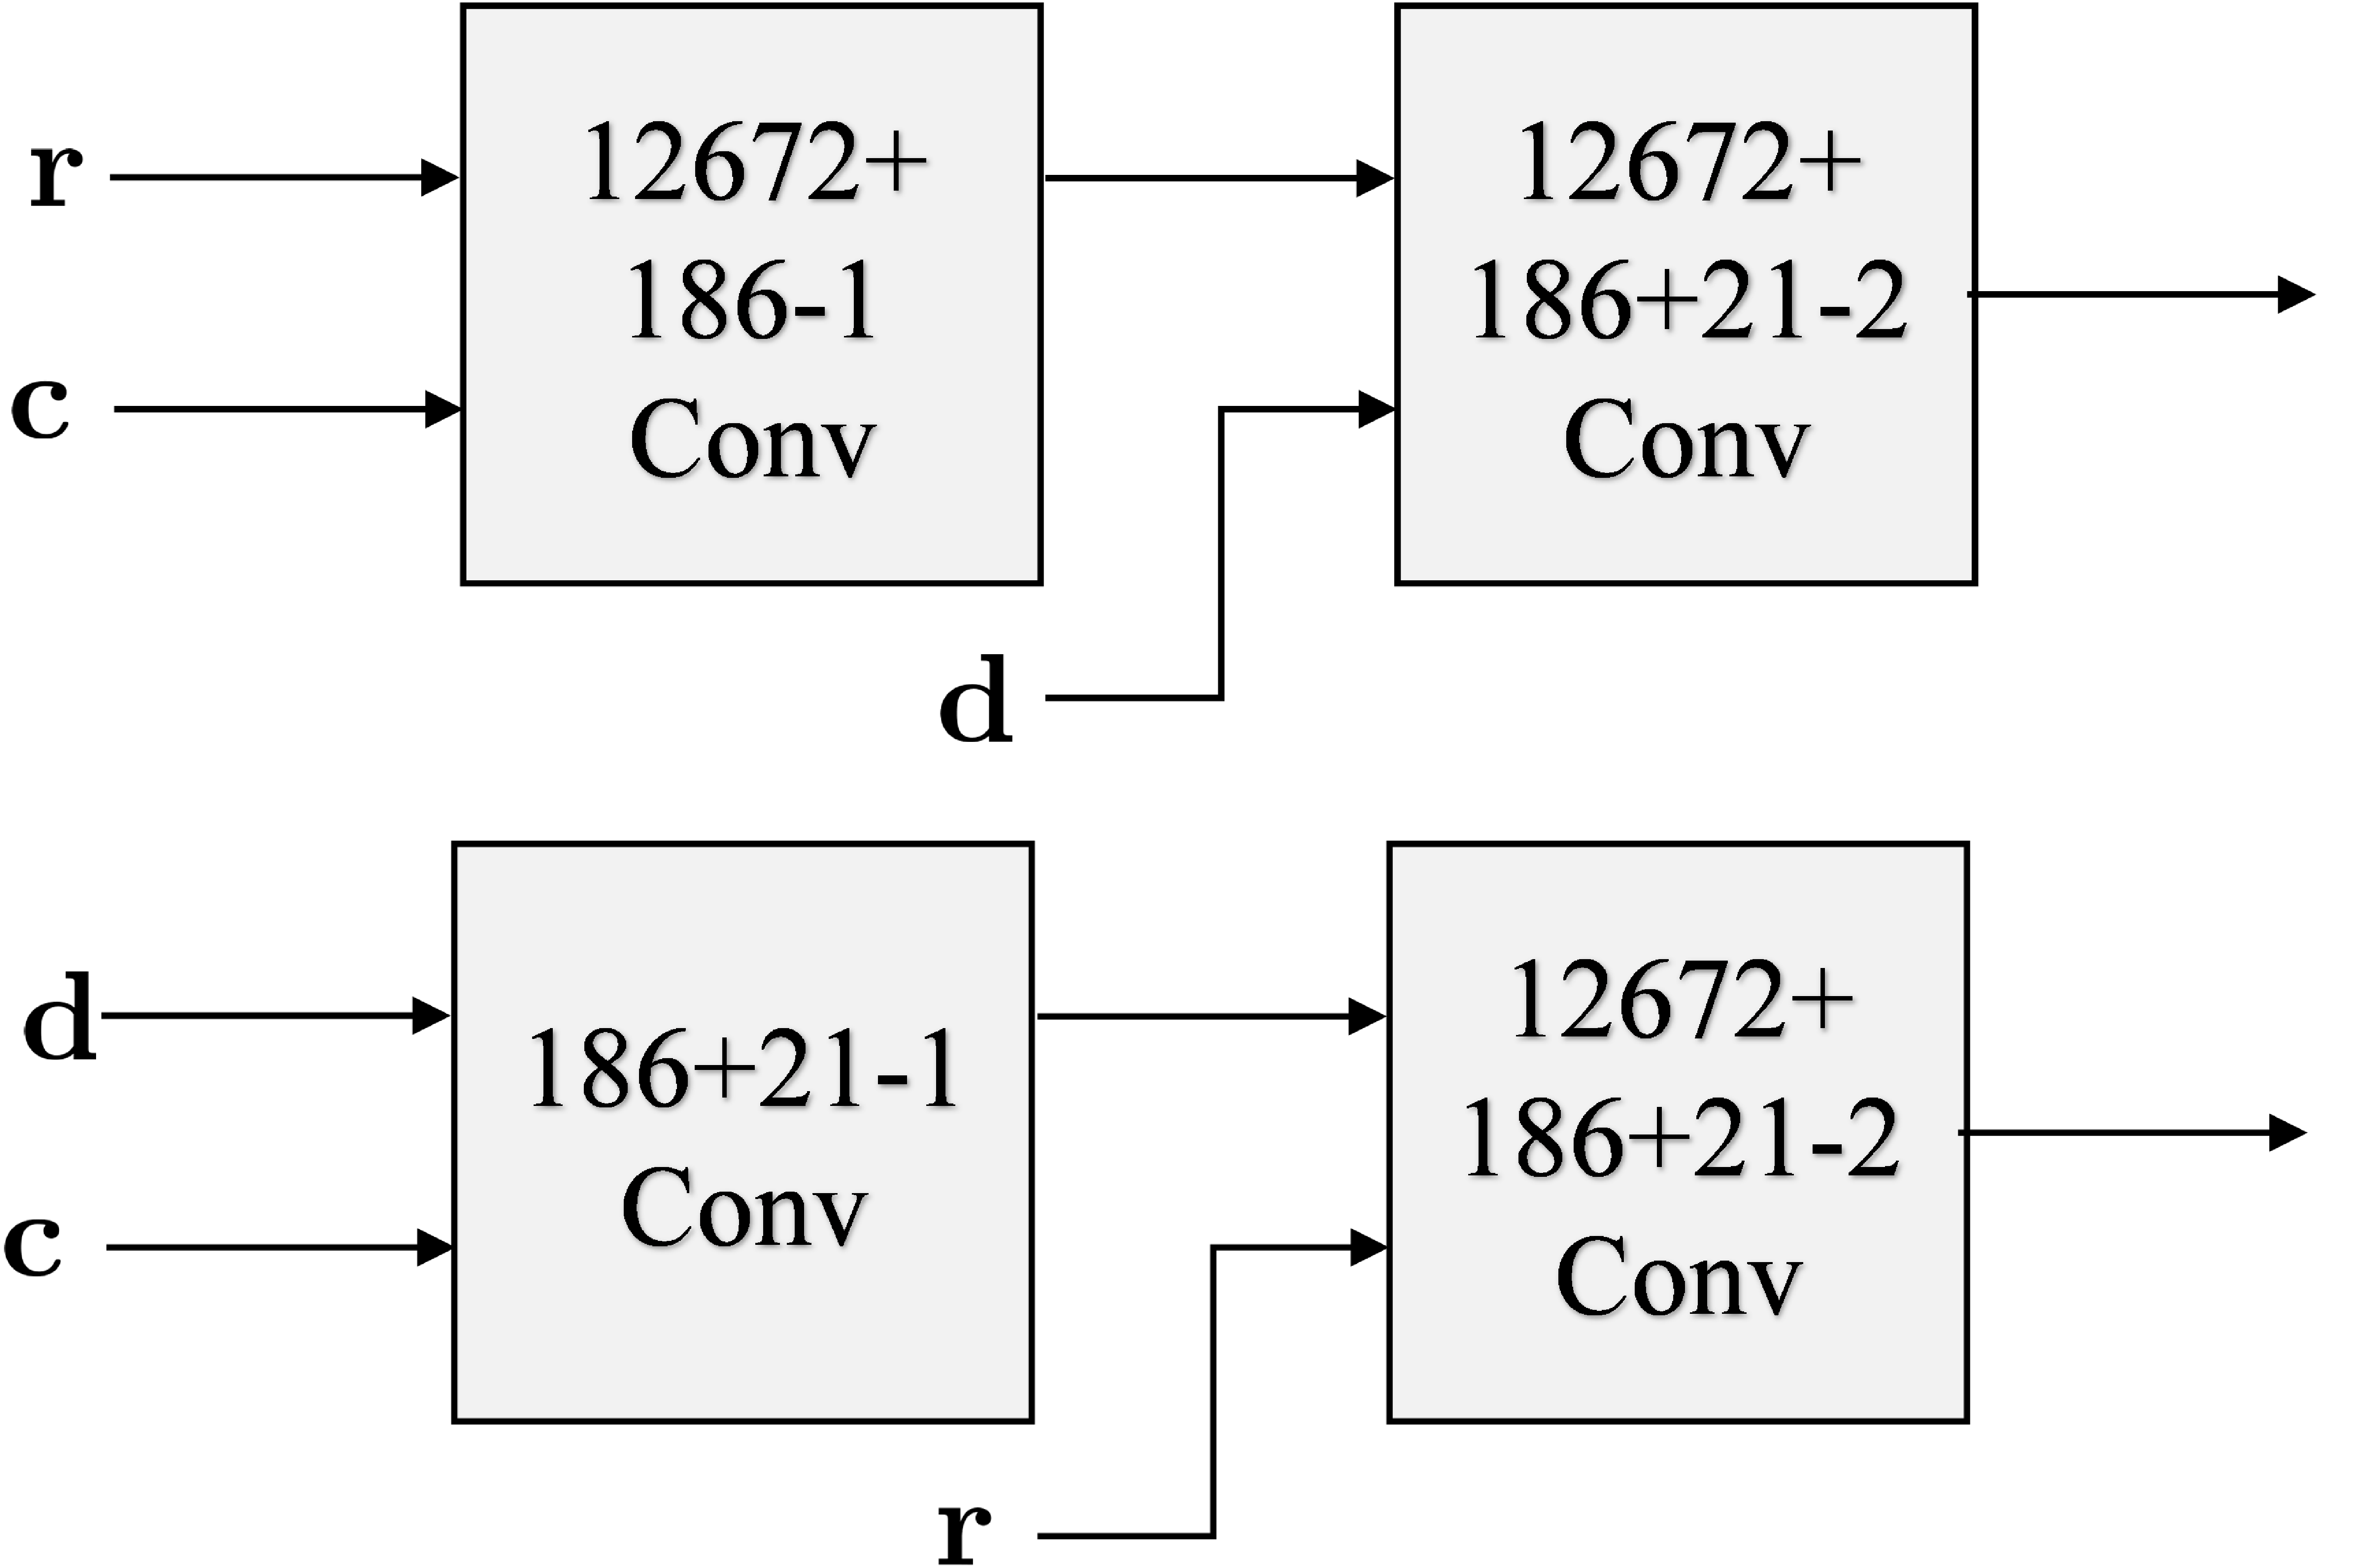
\includegraphics[width=5.01in/100*55]{figures/gpu_intro/twoWaysToConv.pdf}
	\label{fig:twoWaysToConv}
\end{figure}
Figure \ref{fig:twoWaysToConv} shows two ways to cascade the signal $\mathbf{r}$ though two filters.
Rather than applying both filters to the signal, compute a shorter convolution of the $186$ and $21$ tap filters then apply the $186+21-1$ tap result to the signal.

Table \ref{tab:Batched_CPUvsGPUtable_12672_21_186} shows the execution time of implementing cascaded filters, convolving the $21$ and $186$ tap filters is extremely fast in the GPU.
It only costs $2.3165$ms to apply an extra filter in the frequency domain.
It costs $22.0170$ms and $19.7460$ms to apply an extra filter in the time domain because the cascaded filter is now $206$ taps rather than $186$.
Table \ref{tab:Batched_CPUvsGPUtable_12672_206} confirms it costs an extra $20$ms or so to apply a $206$ vs $186$ tap filter.







%%CPUvsGPU_3104batch_21taps_186taps_cascade_varySignal








\section{Cuda Convolution}
Convolution is one of the most important tools in any digital signal processing engineer’s toolbox. 
Convolution can be implemented in the time or frequency domain. 
Theory says if the given filter is ``long'', the frequency domain is the best choice.
But how long is… long? 
First we need a way to measure how computationally intensive an algorithm is. 
The number of floating point operations (flops) is commonly used for benchmarking. 
Let the complex signal length be $N$ and the complex filter length be $L$.
Each complex multiply 
\begin{equation}
(A+jB)\times(C+jD) = (AC-BD)+j(AD+BC)
\end{equation}
is $6$ flops, $4$ multiplies and $2$ additions/subtractions.

Discrete time convolution computed in the time domain is
\begin{equation}
y(n) = \sum^{L-1}_{m=0} x(m) h(n-m).
  \label{eq:simple_conv_time}
\end{equation}
Each output element of $y(n)$ requires a $8L$ flops, $2$ flops (real and imaginary) for each term to be summed then $6$ flops for time signal and filter complex multiply.
The length of the output $\mathbf{y}$ is $N+L-1$.
The number of flops required for convolution of a given length $N$ signal and length $L$ filter is
\begin{equation}
8L(N+L-1) \text{ flops}.
\label{eq:flops_time_domain_conv}
\end{equation}

Discrete time convolution computed in the frequency domain is
\begin{equation}
\mathbf{y} = \mathscr{F}^{-1}(\mathscr{F}(\mathbf{x})\times\mathscr{F}(\mathbf{h})).
  \label{eq:simple_conv_freq}
\end{equation}
The length of the convolution, $M=N+L-1$ is the minimum point Fourier Transform possible.
It is common practice perform a next power of two above the minimum Fourier Transform to leverage the Cooley-Tukey radix 2 Fast Fourier Transform (FFT).
In the Fastest Fourier Transform in the West (FFTW) library the Cooley-Tukey radix 2 transform is used.
Each radix 2 forward or backward Fourier transform performs $5M\log_2(M)$ flops \cite{FFTW:2017,cooley1965algorithm}.
Performing convolution in the frequency domain requires
\begin{equation}
3\times5M\log_2(M)+6M \text{ flops}.
\label{eq:flops_freq_domain_conv}
\end{equation}

\section{Single Convolution}
\label{sec:cuda_convolution_single}
Figure \ref{fig:Theory186Tap_flops} compares the number of flops required for time domain verse frequency domain convolution of a $12672$ sample complex signal with a $186$ tap complex filter.
Figure \ref{fig:Theory21Tap_flops} compares the number of flops required for time domain verse frequency domain convolution of a $12672$ sample complex signal with a $21$ tap complex filter.
Appending zeros to the next power of $2$ causes the stair stepping pattern.
\begin{figure}
	\caption{Comparison of number of floating point operations (flops) required to convolve a $12672$ sample complex signal with a $186$ tap complex filter.}
	\centering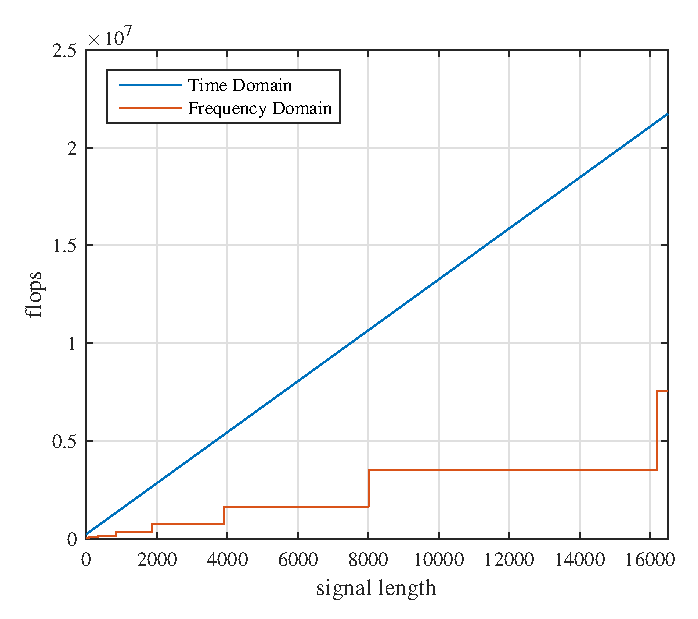
\includegraphics[width=5in]{figures/gpu_intro/Theory186Tap_flops.eps}
	\label{fig:Theory186Tap_flops}
\end{figure}
\begin{figure}
	\caption{Comparison of number of floating point operations (flops) required to convolve a $12672$ sample complex signal with a $21$ tap complex filter.}
	\centering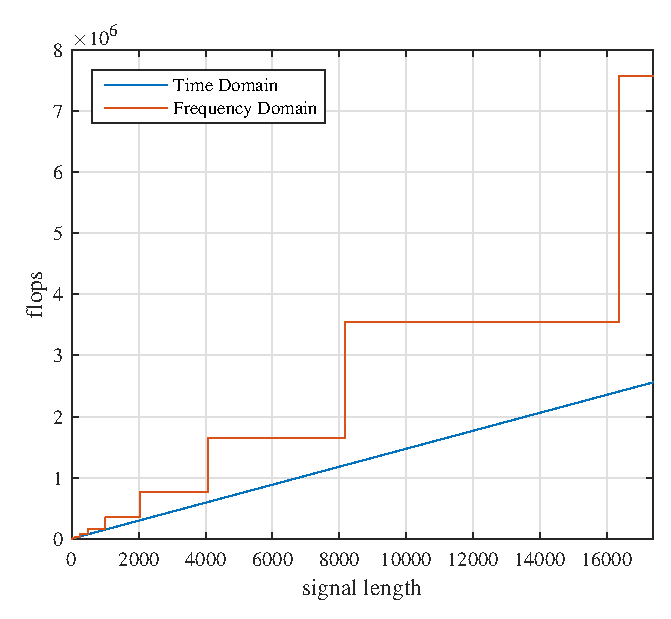
\includegraphics[width=5in]{figures/gpu_intro/Theory21Tap_flops.eps}
	\label{fig:Theory21Tap_flops}
\end{figure}


Now that we understand the number of flops required for a ``short'' filter, does the number of flops affect CPU or GPU execution time?
While Listing \ref{code:GPUvsCPU} is a simple and good example showing how program GPUs, frankly, it is pretty boring and doesn't display the real challenges and tradeoffs of GPUs.
Listing \ref{code:convFun} shows five different ways of implementing convolution:
\begin{itemize}
  \item time domain convolution in a CPU
  \item frequency domain convolution in a CPU
  \item time domain convolution in a GPU using global memory
  \item time domain convolution in a GPU using shared memory
  \item frequency domain convolution in a GPU using CUDA libraries
\end{itemize}
The CPU implements Equation \eqref{eq:simple_conv_time} in ConvCPU directly on line $209$ using a function from lines $11$ to $34$.
The CPU implements Equation \eqref{eq:simple_conv_freq} using the FFTW library on lines $214$ to $258$.
The GPU implements time domain convolution using global memory in lines $268$ to $277$.
The GPU kernel ConvGPU on lines $36$ to $64$ is a parallel version of ConvCPU.
ConvGPU implements time domain convolution by accessing global memory for every element of the signal and filter.
The GPU implements time domain convolution using shared memory in lines $283$ to $292$.
The GPU kernel ConvGPUshared on lines $67$ to $101$ is nearly identical to ConvGPU.
Threads accessing the same elements of the filter in global memory is a waste of valuable clock cycles.
ConvGPUshared pays and initial price on lines $72$ to $76$ to move $L_\text{h}$ filter coefficients from off chip global memory memory to on chip shared memory.
Finally, the GPU implements frequency domain convolution using the cuFFT library on lines $298$ to $326$.


So the questions are:
Do flops have a direct relationship to execution time on CPUs? 
Do flops have a direct relationship to execution time on GPUs? 
When is convolution in CPUs faster than GPUs?
When is it worth the initial cost to used shared memory?
When should convolution be done in the frequency domain?

The answer to all of the questions is...it depends on your signal length, filter length, CPU, GPU and memory.
A CUDA programmer can make an educated guess on which algorithm may be faster, but until all the algorithms have been implemented and timed, there is no definite answer.

To demonstrate that there is no definite answer in GPUs, 
the execution time of the code in Listing \ref{code:GPUvsCPU} was timed.
Only the CPU functions were timed for the time and frequency domain convolution on the CPU.
Each memory transfer host to device and device to host was timed for a fair comparison of GPU to CPU.
Table \ref{tab:CPUvsGPUtimingTable} shows where timing was started and stopped for each algorithm.
\begin{table}
\caption{Defining start and stop lines for timing comparison in Listing \ref{code:convFun}.}
\begin{center}
\begin{tabular}{llll}
	\toprule
	Algorithm 				& Function		& Start Line	& Stop  Line		\\ \midrule
	CPU time domain 		& ConvCPU 		& 208			& 210 				\\
	CPU frequency domain 	& FFTW 			& 213			& 259 				\\
	GPU time domain global 	& ConvGPU 		& 267			& 278				\\
	GPU time domain shared 	& ConvGPUshared & 282			& 293				\\
	GPU frequency domain 	& cuFFT			& 301			& 327				\\ 
	\bottomrule
\end{tabular}
\end{center}
\label{tab:CPUvsGPUtimingTable}
\end{table}

Figure \ref{fig:CPUvsGPU_1batch_186taps_varySignal_noMin} compares the computation time of a fixed length $186$ tap filter convolved with a varied length signal.
The execution time varies enough that the plot is messy and unreadable.
Figure \ref{fig:CPUvsGPU_1batch_186taps_varySignal} compares the same data but $15$ sample local minimums were found.
\begin{figure}
	\caption{Comparison of a complex convolution on CPU verse GPU. The signal length is varied and the filter is fixed at $186$ taps. The comparison is messy with out lower bounding.}
	\centering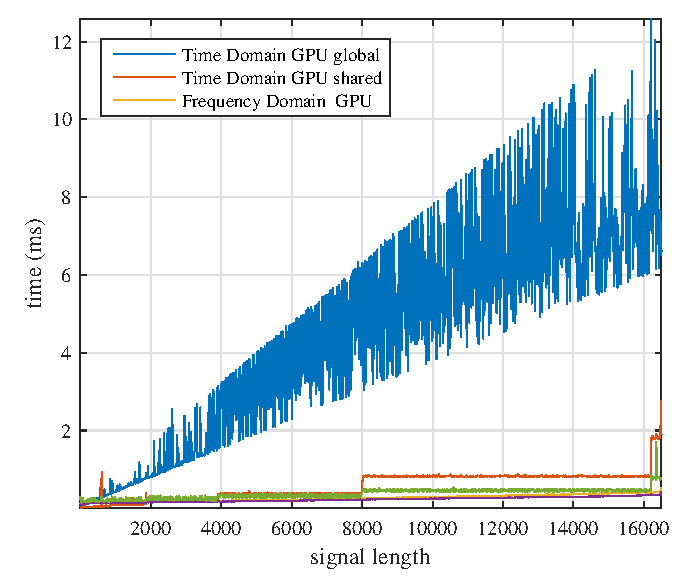
\includegraphics[width=5in]{figures/gpu_intro/CPUvsGPU_1batch_186taps_varySignal_noMin.eps}
	\label{fig:CPUvsGPU_1batch_186taps_varySignal_noMin}
\end{figure}
\begin{figure}
	\caption{Comparison of a complex convolution on CPU verse GPU. The signal length is varied and the filter is fixed at $186$ taps. A lower bound was applied by searching for a local minimums in $15$ sample width windows.}
	\centering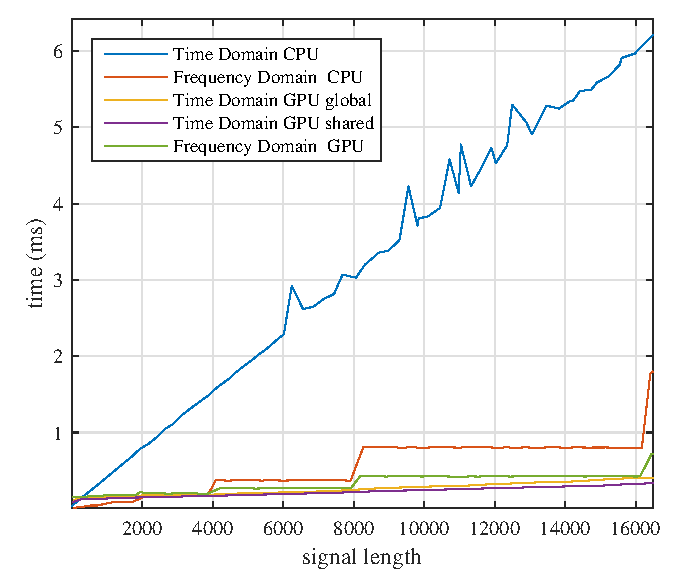
\includegraphics[width=5in]{figures/gpu_intro/CPUvsGPU_1batch_186taps_varySignal.eps}
	\label{fig:CPUvsGPU_1batch_186taps_varySignal}
\end{figure}

With the plot lower bounded, compare Figure \ref{fig:CPUvsGPU_1batch_186taps_varySignal} to Figure \ref{fig:Theory186Tap_flops}.
Does the CPU and GPU follow the same trend as the number of flops?
The CPU has the exact structure that the number of flops predicted.
The GPU does have the stair stepping from appending zeros for the frequency domain, but the time domain GPU kernels execute in less time.

The GPU execution time does not follow the same trend as the number of flops.
Why? As mentioned in Section \ref{sec:GPU_memory}, GPUs have a hanes amount of computational resources and limited memory bandwidth.
Over $90\%$ of GPU kernels are memory bandwidth limited.

To provide more proof, compare Figures \ref{fig:CPUvsGPU_1batch_21taps_varySignal} and \ref{fig:Theory21Tap_flops}.
Once again, the CPU follows the same trend as the number of flops.
The GPU also follows the number of flops trends but to a lesser extent than the CPU.
On ``short'' filters, using shared memory will perform better than using only global memory.
Using shared memory to store the short filter saves the each iteration a lot of execution time.
\begin{figure}
	\caption{Comparison of a complex convolution on CPU verse GPU. The signal length is varied and the filter is fixed at $21$ taps. A lower bound was applied by searching for a local minimums in $5$ sample width windows.}
	\centering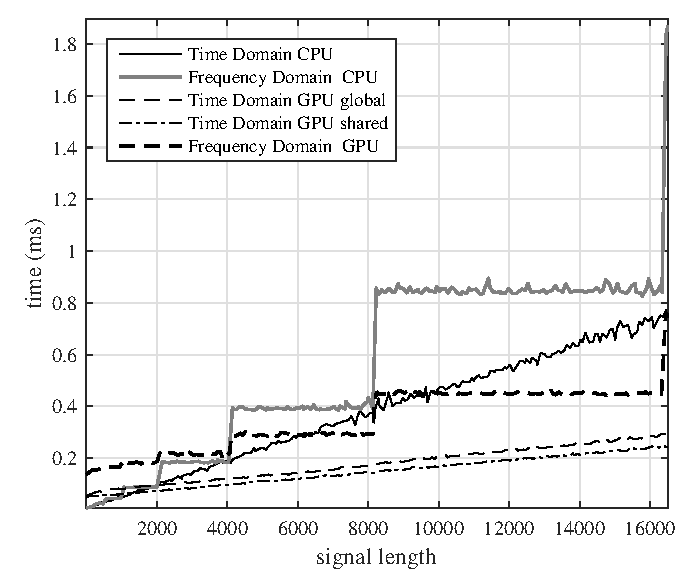
\includegraphics[width=5in]{figures/gpu_intro/CPUvsGPU_1batch_21taps_varySignal.eps}
	\label{fig:CPUvsGPU_1batch_21taps_varySignal}
\end{figure}

What if the signal length was set and the filter length was varied?
Figure \ref{fig:CPUvsGPU_1batch_12672signal_varyFilter} compares CPU to GPU execution time of a $12672$ sample signal convolved with a varying filter length.
The time domain CPU execution time is affected obviously because the number of flops increases.

Neither CPU or GPU frequency domain execution time is affected by varying filter length.
The execution time stays the same because the number of memory accesses and flops remain constant because the filter is appended with zeros to the convolution length.

The execution time of both time domain GPU convolutions are slightly affected by increasing filter length.
The number of memory accesses per output sample increase as the filter length increases.
Bottom line, the length of the signal is the largest factor as Equations \ref{eq:flops_time_domain_conv} and \ref{eq:flops_freq_domain_conv} suggest.
\begin{figure}
	\caption{Comparison of a complex convolution on CPU verse GPU. The filter length is varied and the signal is fixed at $12672$ samples. A lower bound was applied by searching for a local minimums in $3$ sample width windows.}
	\centering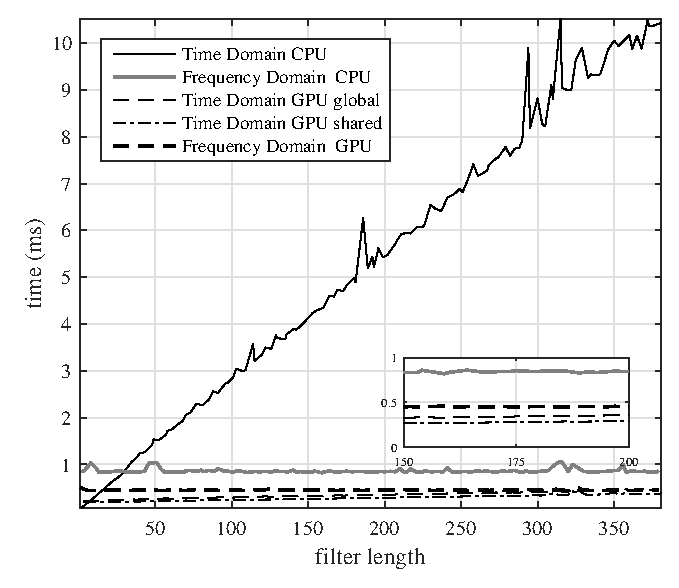
\includegraphics[width=5in]{figures/gpu_intro/CPUvsGPU_1batch_12672signal_varyFilter.eps}
	\label{fig:CPUvsGPU_1batch_12672signal_varyFilter}
\end{figure}

Conclusion, when needing implement convolution in a CPU or GPU, implement it every way possible.
Which ever way has the fastest execution time, he is your winner.
Long story short, most of the time a GPU DSP engineer is given a set length for the signal and filter.
As Figures \ref{fig:CPUvsGPU_1batch_186taps_varySignal_noMin} through \ref{fig:CPUvsGPU_1batch_12672signal_varyFilter} have shown, unless every implementation is explored, there is no way of saying which implementation will absolutely be fastest.

Table \ref{tab:CPUvsGPUtable_12672_186} shows GPU frequency domain is fastest when convolving a $12672$ sample signal with a $186$ tap filter.
Table \ref{tab:CPUvsGPUtable_12672_21} shows GPU time domain using shared is fastest when convolving a $12672$ sample signal with a $21$ tap filter.
\begin{table}
\caption{Convolution computation times with signal length $12672$ and filter length $186$ on a Tesla K40c GPU.}
\begin{center}
\begin{tabular}{lll}
	\toprule
	Algorithm 				& Function or Library		& Execution Time (ms) \\ \midrule
	CPU time domain 		& ConvCPU 					& 5.0388		\\
	CPU frequency domain 	& FFTW 						& 1.6295		\\
	GPU time domain global 	& ConvGPU 					& 0.4021		\\
	GPU time domain shared 	& ConvGPUshared 			& 0.3752		\\
	GPU frequency domain 	& cuFFT						& 0.3387		\\ 
	\bottomrule
\end{tabular}
\end{center}
\label{tab:CPUvsGPUtable_12672_186}
\end{table}
\begin{table}
\caption{Convolution computation times with signal length $12672$ and filter length $21$ on a Tesla K40c GPU.}
\begin{center}
\begin{tabular}{lll}
	\toprule
	Algorithm 				& Function or Library		& Execution Time (ms) \\ \midrule
	CPU time domain 		& ConvCPU 					& 0.6125		\\
	CPU frequency domain 	& FFTW 						& 2.5947		\\
	GPU time domain global 	& ConvGPU 					& 0.2405		\\
	GPU time domain shared 	& ConvGPUshared 			& 0.2112		\\
	GPU frequency domain 	& cuFFT						& 0.3360		\\ 
	\bottomrule
\end{tabular}
\end{center}
\label{tab:CPUvsGPUtable_12672_21}
\end{table}

\section{Batched Convolution}
In section \ref{sec:cuda_convolution_single} convolution of a single single with a single filter was studied.
Chapter blah (system overview) shows the packetized structure of the received signal.
The received signal has $3104$ packets or batches and each packet is independent of other packets.

Now that we have $3104$ signals to be convolved with $3104$ filters, how does the problem change?
Which approach to convolution will be fastest?

As the number of batches increases, does CPU and GPU execution time increase linearly?
Figure \ref{fig:CPUvsGPU_varyBatches_186taps_12672signal} shows how the execution time increases with the number of batches.
Note that no lower bounding is needed to produce clean batched processing results.
This figure shows that frequency domain convolution leverages batch processing better than time domain convolution.
No surprise CPU time and frequency domain execution time skyrockets as the number of batches increases.
The GPU handles batched processing very well because it introduces more parallelism.
\begin{figure}
	\caption{Comparison of a batched complex convolution on a CPU and GPU. The number of batches is varied while the signal and filter length is set to $12672$ and $186$.}
	\centering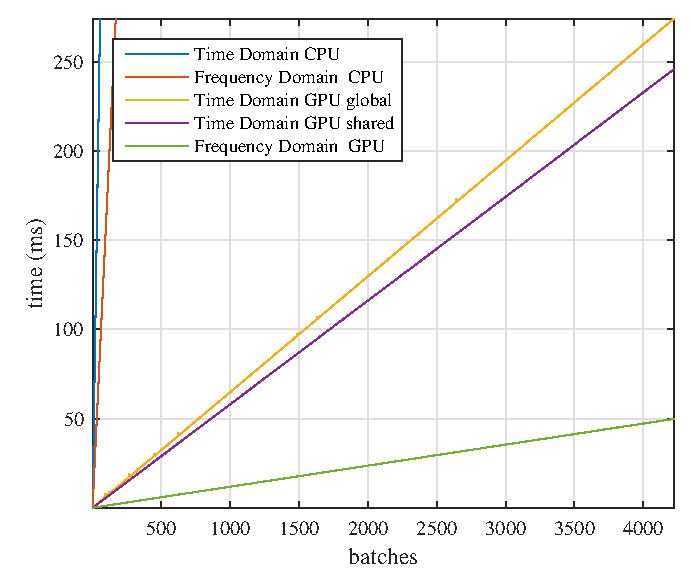
\includegraphics[width=5in]{figures/gpu_intro/CPUvsGPU_varyBatches_186taps_12672signal.eps}
	\label{fig:CPUvsGPU_varyBatches_186taps_12672signal}
\end{figure}

Judging by Figure \ref{fig:CPUvsGPU_varyBatches_186taps_12672signal}, CPU is not a contender in batched processing for fast execution times when compared to the GPU.
CPU and GPU batched processing will not be compared any further.
Listing \ref{code:batchedConvFun} shows three ways of batched convolution in CUDA
\begin{itemize}
  \item time domain convolution in a GPU using global memory
  \item time domain convolution in a GPU using shared memory
  \item frequency domain convolution in a GPU using the cuFFT library.
\end{itemize}

Now that the GPU execution time isn't being compared to the CPU, transfers between host and device will not be a factor for algorithm comparison.
Table \ref{tab:BatchedGPUtimingTable} shows how Listing \ref{code:batchedConvFun} is timed.
\begin{table}
\caption{Defining start and stop lines for timing comparison in Listing \ref{code:batchedConvFun}.}
\begin{center}
\begin{tabular}{llll}
	\toprule
	Algorithm 				& Function		& Start Line	& Stop  Line		\\ \midrule
	GPU time domain global 	& ConvGPU 		& 197			& 204				\\
	GPU time domain shared 	& ConvGPUshared & 212			& 219				\\
	GPU frequency domain 	& cuFFT			& 227			& 245				\\ 
	\bottomrule
\end{tabular}
\end{center}
\label{tab:BatchedGPUtimingTable}
\end{table}


Figure \ref{fig:CPUvsGPU_3104batch_186taps_varySignal} shows execution time for $3104$ batches of $186$ tap filters convolved with varying signal lengths.
Performing frequency domain convolution is always faster than time domain convolution because the cuFFT library is better optimized for batched processing.
Frequency domain convolution for a $12672$ sample signal takes just $36.8$ms, that is on average $0.0119$ms per batch.
Compare $0.0119$ms per batch to single batched execution time in Table \ref{tab:CPUvsGPUtable_12672_186}, one batch took $0.3387$.
Batched processing introduced a $28\times$ speed up!
\begin{figure}
	\caption{Comparison of a batched complex convolution on a GPU. The signal length is varied and the filter is fixed at $186$ taps.}
	\centering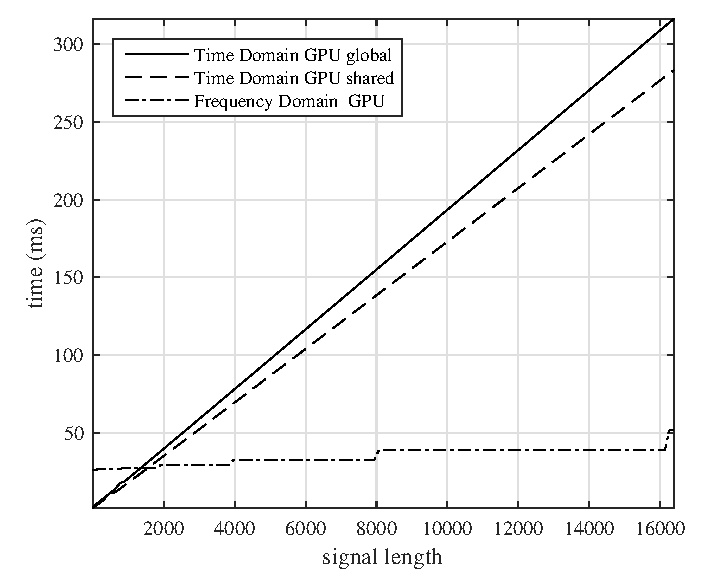
\includegraphics[width=5in]{figures/gpu_intro/CPUvsGPU_3104batch_186taps_varySignal.eps}
	\label{fig:CPUvsGPU_3104batch_186taps_varySignal}
\end{figure}

Figure \ref{fig:CPUvsGPU_3104batch_21taps_varySignal} shows execution time for $3104$ batches of $21$ tap filters convolved with varying signal lengths.
This figure exhibits the same characteristics of single batch convolution execution time shown in Figure \ref{fig:CPUvsGPU_1batch_21taps_varySignal}.
For most signal lengths, performing time domain convolution using shared memory is fastest.
\begin{figure}
	\caption{Comparison of a batched complex convolution on a GPU. The signal length is varied and the filter is fixed at $21$ taps.}
	\centering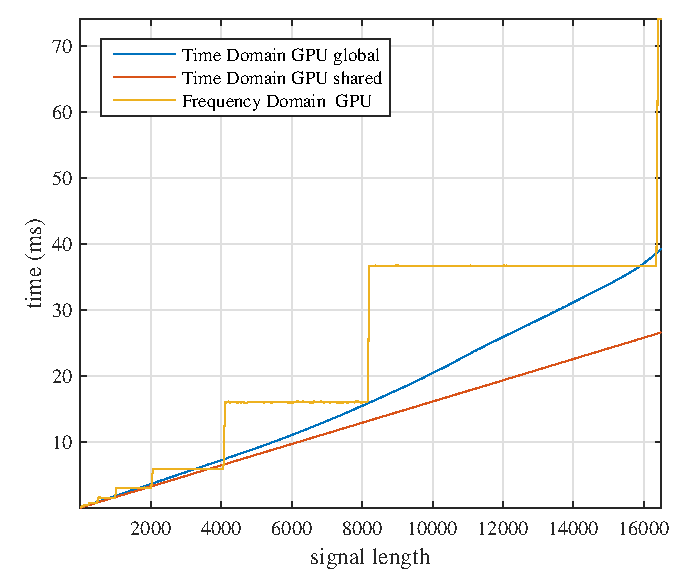
\includegraphics[width=5in]{figures/gpu_intro/CPUvsGPU_3104batch_21taps_varySignal.eps}
	\label{fig:CPUvsGPU_3104batch_21taps_varySignal}
\end{figure}

Figure \ref{fig:CPUvsGPU_3104batch_12672signal_varyFilter} shows execution time for $3104$ batches of $12672$ sample signal convolved with varying filter lengths.
This figure exhibits nearly the same characteristics of single batch convolution execution time shown in Figure \ref{fig:CPUvsGPU_1batch_12672signal_varyFilter} accept the varied filter length has no affect on execution time.
For very short filter lengths, time domain convolution using shared memory is fastest.
For longer filters , frequency domain convolution is fastest.
\begin{figure}
	\caption{Comparison of a batched complex convolution on a GPU. The signal length is varied and the filter is fixed at $21$ taps.}
	\centering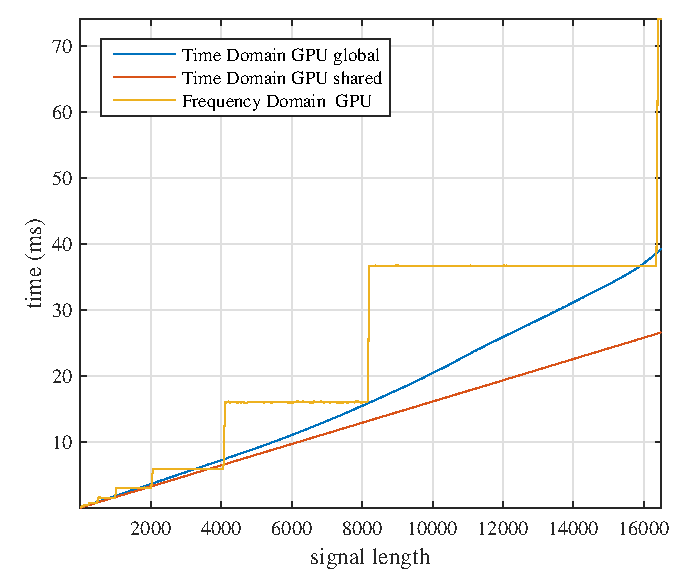
\includegraphics[width=5in]{figures/gpu_intro/CPUvsGPU_3104batch_21taps_varySignal.eps}
	\label{fig:CPUvsGPU_3104batch_21taps_varySignal}
\end{figure}

Though this section has show that in batched processing the algorithm leading to the fastest execution time still depends on signal and filter length,
one important comcept has been over looked.
Figure \ref{fig:ProcessingBlock} shows there are two filters that need to be allied to the signal. 

If convolution is implemented in the time domain, ConvGPU or ConvGPUshared must run twice.
The first call of ConvGPU or ConvGPUshared performs the convolution of the $186$ tap equalizer and $21$ detection filter.
The second call of ConvGPU or ConvGPUshared performs the convolution of the $12672$ sample signal with the  convolved $186+21-1$ tap filter.

If convolution is implemented in the frequency domain, only the GPU kernel PointToPointMultiply has to be updated.
PointToPointMultiply must be changed from two input vectors to three input vectors.
For every point the number of memory accesses increases by $1$ element and the number of flops doubles from $6$ to $12$.
An extra cuFFT call would be expected accept the detection filter in Figure \ref{fig:ProcessingBlock} constant.
The FFT of the detection filter can be calculated and stored at initialization.

Table \ref{tab:Batched_CPUvsGPUtable_12672_186} shows the batched convolution execution time for a $12672$ sample signal and $186$ tap filter.
Table \ref{tab:Batched_CPUvsGPUtable_12672_21} shows the batched convolution execution time for a $12672$ sample signal and $21$ tap filter.
Table \ref{tab:Batched_CPUvsGPUtable_12672_21_186} shows the batched cascaded convolution execution time for a $12672$ sample signal with $21$ and $186$ tap filters.
\begin{table}
\caption{Batched convolution execution times with for a $12672$ sample signal and $186$ tap filter on a Tesla K40c GPU.}
\begin{center}
\begin{tabular}{lll}
	\toprule
	Algorithm 				& Function or Library		& Execution Time (ms) \\ \midrule
	GPU time domain global 	& ConvGPU 					& 201.29		\\
	GPU time domain shared 	& ConvGPUshared 			& 180.272		\\
	GPU frequency domain 	& cuFFT						& 36.798 		\\ 
	\bottomrule
\end{tabular}
\end{center}
\label{tab:Batched_CPUvsGPUtable_12672_186}
\end{table}
\begin{table}
\caption{Batched convolution execution times with for a $12672$ sample signal and $21$ tap filter on a Tesla K40c GPU.}
\begin{center}
\begin{tabular}{lll}
	\toprule
	Algorithm 				& Function or Library		& Execution Time (ms) \\ \midrule
	GPU time domain global 	& ConvGPU 					& 27.642		\\
	GPU time domain shared 	& ConvGPUshared 			& 20.4287		\\
	GPU frequency domain 	& cuFFT						& 36.7604		\\ 
	\bottomrule
\end{tabular}
\end{center}
\label{tab:Batched_CPUvsGPUtable_12672_21}
\end{table}
\begin{table}
\caption{Batched convolution execution times with for a $12672$ sample signal and $206$ tap filter on a Tesla K40c GPU.}
\begin{center}
\begin{tabular}{lll}
	\toprule
	Algorithm 				& Function or Library		& Execution Time (ms) \\ \midrule
	GPU time domain global 	& ConvGPU 					& 223.064		\\
	GPU time domain shared 	& ConvGPUshared 			& 199.844		\\
	GPU frequency domain 	& cuFFT						& 36.7704		\\ 
	\bottomrule
\end{tabular}
\end{center}
\label{tab:Batched_CPUvsGPUtable_12672_206}
\end{table}
\begin{table}
\caption{Batched convolution execution times with for a $12672$ sample signal and cascaded $21$ and $186$ tap filter on a Tesla K40c GPU.}
\begin{center}
\begin{tabular}{lll}
	\toprule
	Algorithm 				& Function or Library		& Execution Time (ms) \\ \midrule
	GPU time domain global 	& ConvGPU 					& 223.307		\\
	GPU time domain shared 	& ConvGPUshared 			& 200.018		\\
	GPU frequency domain 	& cuFFT						& 39.0769		\\ 
	\bottomrule
\end{tabular}
\end{center}
\label{tab:Batched_CPUvsGPUtable_12672_21_186}
\end{table}

Tables \ref{tab:Batched_CPUvsGPUtable_12672_186} and \ref{tab:Batched_CPUvsGPUtable_12672_21} agree with Figures \ref{fig:CPUvsGPU_3104batch_21taps_varySignal} and \ref{fig:CPUvsGPU_3104batch_186taps_varySignal}.
Time domain convolution is faster with a short $21$ tap filter but frequency domain convolution is faster with a long $186$ tap filter.

\begin{figure}
	\caption{Two ways to convolve the signal $\mathbf{r}$ with the $186$ tap filter $\mathbf{c}$ and $21$ tap filter $\mathbf{d}$.}
	\centering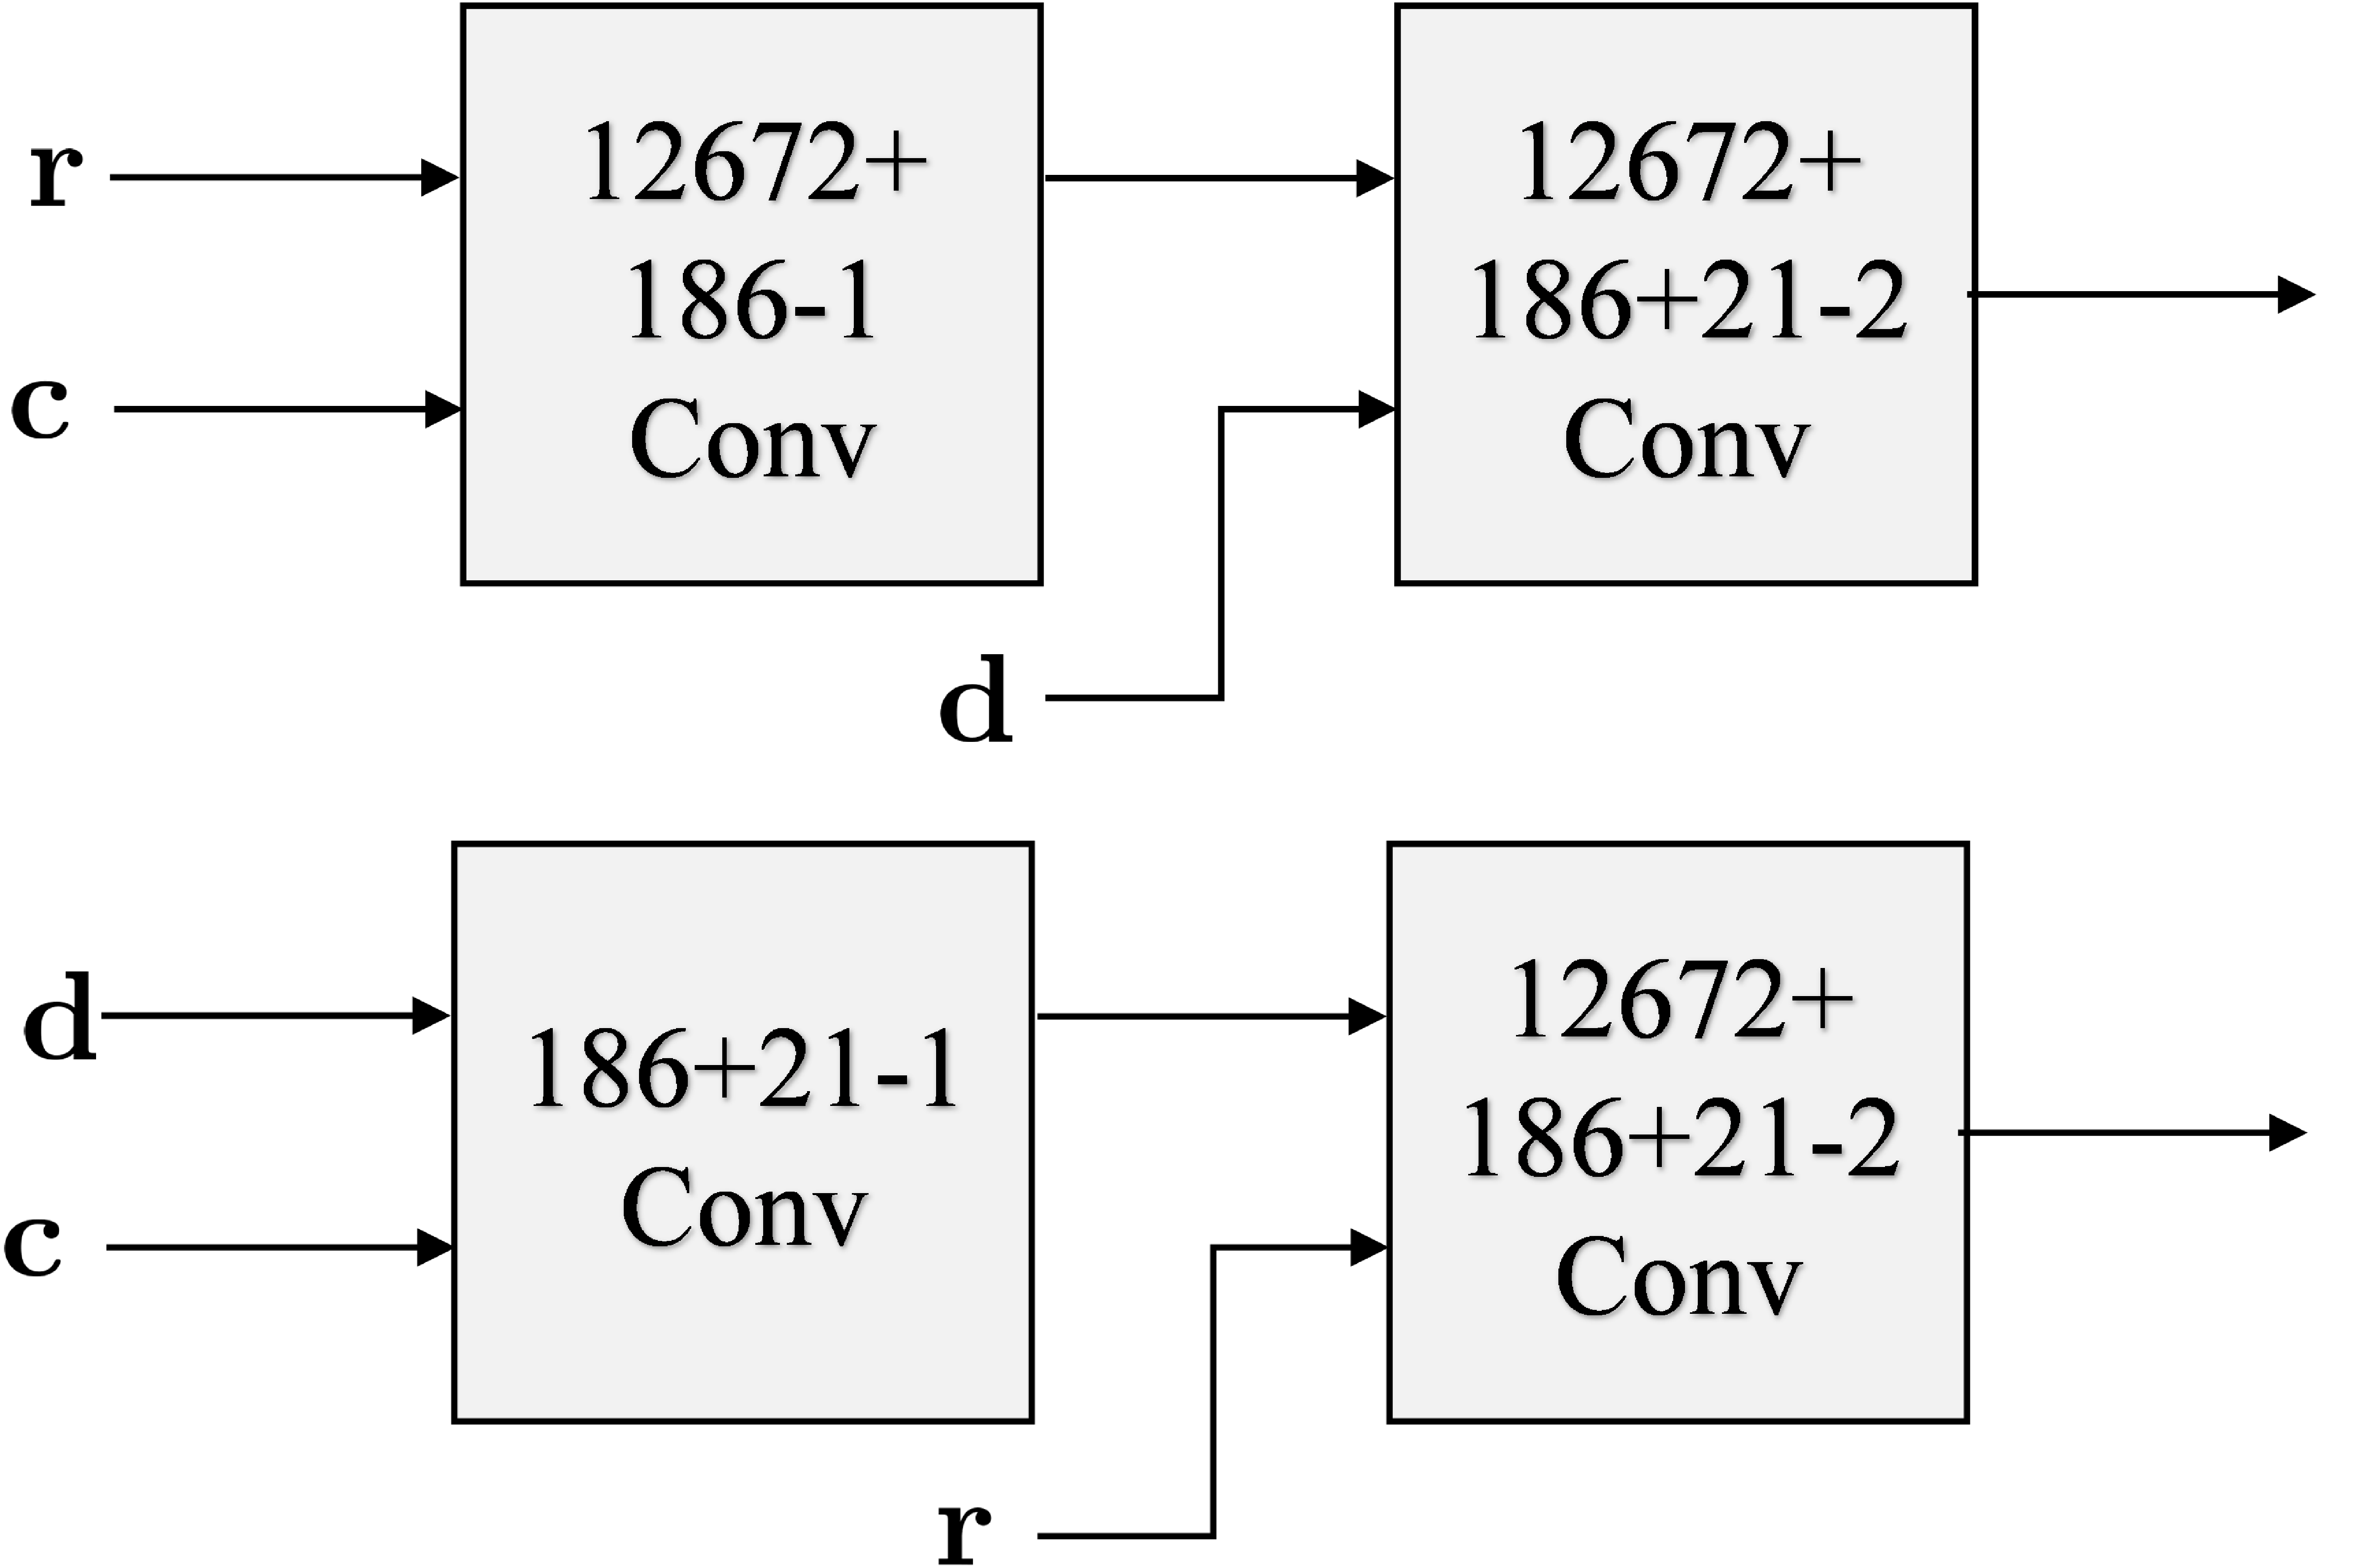
\includegraphics[width=5.01in/100*55]{figures/gpu_intro/twoWaysToConv.pdf}
	\label{fig:twoWaysToConv}
\end{figure}
Figure \ref{fig:twoWaysToConv} shows two ways to cascade the signal $\mathbf{r}$ though two filters.
Rather than applying both filters to the signal, compute a shorter convolution of the $186$ and $21$ tap filters then apply the $186+21-1$ tap result to the signal.

Table \ref{tab:Batched_CPUvsGPUtable_12672_21_186} shows the execution time of implementing cascaded filters, convolving the $21$ and $186$ tap filters is extremely fast in the GPU.
It only costs $2.3165$ms to apply an extra filter in the frequency domain.
It costs $22.0170$ms and $19.7460$ms to apply an extra filter in the time domain because the cascaded filter is now $206$ taps rather than $186$.
Table \ref{tab:Batched_CPUvsGPUtable_12672_206} confirms it costs an extra $20$ms or so to apply a $206$ vs $186$ tap filter.

Figure \ref{fig:CPUvsGPU_3104batch_21taps_186taps_cascade_varySignal} shows 
\begin{figure}
	\caption{Comparison of a batched cascaded complex convolution on a GPU. The signal length is varied and the filter is the $206$ result of convolving $186$ and $21$ tap filters.}
	\centering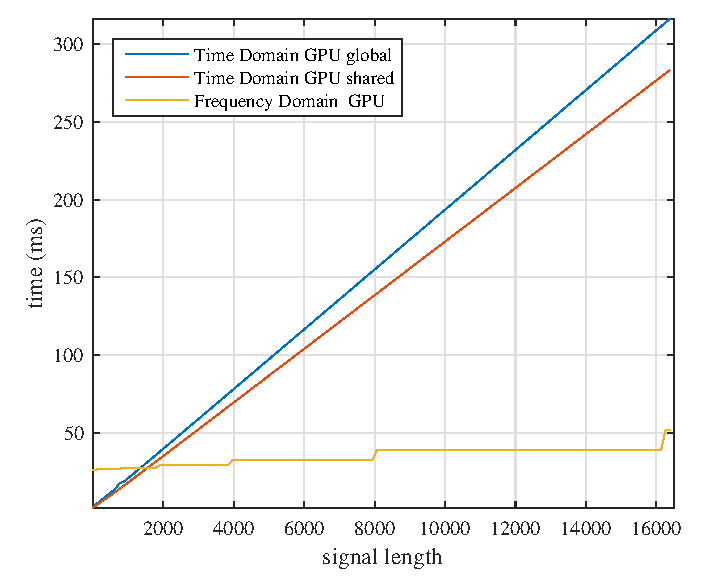
\includegraphics[width=5in]{figures/gpu_intro/CPUvsGPU_3104batch_21taps_186taps_cascade_varySignal.eps}
	\label{fig:CPUvsGPU_3104batch_21taps_186taps_cascade_varySignal}
\end{figure}


\singlespacing
\clearpage
\begin{lstlisting}[style=myCUDAstyle,language=C++,caption={CUDA code to performing complex convolution five different ways: time domain CPU, frequency domain CPU time domain GPU, time domain GPU using shared memory and frequency domain GPU.},label={code:convFun}]
#include <iostream>
#include <stdlib.h>
#include <math.h>
#include <cufft.h>
#include <fstream>
#include <string>
#include <fftw3.h>
using namespace std;


void ConvCPU(cufftComplex* y,cufftComplex* x,cufftComplex* h,int Lx,int Lh){
	for(int yIdx = 0; yIdx < Lx+Lh-1; yIdx++){
		cufftComplex temp;
		temp.x = 0;
		temp.y = 0;
		for(int hIdx = 0; hIdx < Lh; hIdx++){
			int xAccessIdx = yIdx-hIdx;
			if(xAccessIdx>=0 && xAccessIdx<Lx){
				// temp += x[xAccessIdx]*h[hIdx];
				float A = x[xAccessIdx].x;
				float B = x[xAccessIdx].y;
				float C = h[hIdx].x;
				float D = h[hIdx].y;
				cufftComplex result;
				result.x = A*C-B*D;
				result.y = A*D+B*C;
				temp.x += result.x;
				temp.y += result.y;
			}
		}
		y[yIdx] = temp;
	}

}

__global__ void ConvGPU(cufftComplex* y,cufftComplex* x,cufftComplex* h,int Lx,int Lh){
	int yIdx = blockIdx.x*blockDim.x + threadIdx.x;

	int lastThread = Lx+Lh-1;

	// don't access elements out of bounds
	if(yIdx >= lastThread)
		return;

	cufftComplex temp;
	temp.x = 0;
	temp.y = 0;
	for(int hIdx = 0; hIdx < Lh; hIdx++){
		int xAccessIdx = yIdx-hIdx;
		if(xAccessIdx>=0 && xAccessIdx<Lx){
			// temp += x[xAccessIdx]*h[hIdx];
			float A = x[xAccessIdx].x;
			float B = x[xAccessIdx].y;
			float C = h[hIdx].x;
			float D = h[hIdx].y;
			cufftComplex result;
			result.x = A*C-B*D;
			result.y = A*D+B*C;
			temp.x += result.x;
			temp.y += result.y;
		}
	}
	y[yIdx] = temp;
}


__global__ void ConvGPUshared(cufftComplex* y,cufftComplex* x,cufftComplex* h,int Lx,int Lh){
	int yIdx = blockIdx.x*blockDim.x + threadIdx.x;

	int lastThread = Lx+Lh-1;

	extern __shared__ cufftComplex h_shared[];
	if(threadIdx.x < Lh){
		h_shared[threadIdx.x] = h[threadIdx.x];
	}
	__syncthreads();

	// don't access elements out of bounds
	if(yIdx >= lastThread)
		return;

	cufftComplex temp;
	temp.x = 0;
	temp.y = 0;
	for(int hIdx = 0; hIdx < Lh; hIdx++){
		int xAccessIdx = yIdx-hIdx;
		if(xAccessIdx>=0 && xAccessIdx<Lx){
			// temp += x[xAccessIdx]*h[hIdx];
			float A = x[xAccessIdx].x;
			float B = x[xAccessIdx].y;
			float C = h_shared[hIdx].x;
			float D = h_shared[hIdx].y;
			cufftComplex result;
			result.x = A*C-B*D;
			result.y = A*D+B*C;
			temp.x += result.x;
			temp.y += result.y;
		}
	}
	y[yIdx] = temp;
}

__global__ void PointToPointMultiply(cufftComplex* v0, cufftComplex* v1, int lastThread){
	int i = blockIdx.x*blockDim.x + threadIdx.x;

	// don't access elements out of bounds
	if(i >= lastThread)
		return;
	float A = v0[i].x;
	float B = v0[i].y;
	float C = v1[i].x;
	float D = v1[i].y;

	// (A+jB)(C+jD) = (AC-BD) + j(AD+BC)
	cufftComplex result;
	result.x = A*C-B*D;
	result.y = A*D+B*C;

	v0[i] = result;
}

__global__ void ScalarMultiply(cufftComplex* vec0, float scalar, int lastThread){
	int i = blockIdx.x*blockDim.x + threadIdx.x;

	// Don't access elements out of bounds
	if(i >= lastThread)
		return;
	cufftComplex scalarMult;
	scalarMult.x = vec0[i].x*scalar;
	scalarMult.y = vec0[i].y*scalar;
	vec0[i] = scalarMult;
}

int main(){
	int mySignalLength = 1000;
	int myFilterLength = 186;
	int myConvLength   = mySignalLength + myFilterLength - 1;
	int Nfft           = pow(2, ceil(log(myConvLength)/log(2)));

	cufftComplex *mySignal1;
	cufftComplex *mySignal2;
	cufftComplex *mySignal2_fft;

	cufftComplex *myFilter1;
	cufftComplex *myFilter2;
	cufftComplex *myFilter2_fft;

	cufftComplex *myConv1;
	cufftComplex *myConv2;
	cufftComplex *myConv2_timeReversed;
	cufftComplex *myConv3;
	cufftComplex *myConv4;
	cufftComplex *myConv5;

	mySignal1      		= (cufftComplex*)malloc(mySignalLength*sizeof(cufftComplex));
	mySignal2      		= (cufftComplex*)malloc(Nfft  		  *sizeof(cufftComplex));
	mySignal2_fft  		= (cufftComplex*)malloc(Nfft   	      *sizeof(cufftComplex));

	myFilter1      		= (cufftComplex*)malloc(myFilterLength*sizeof(cufftComplex));
	myFilter2      		= (cufftComplex*)malloc(Nfft   	      *sizeof(cufftComplex));
	myFilter2_fft  		= (cufftComplex*)malloc(Nfft  		  *sizeof(cufftComplex));

	myConv1        		= (cufftComplex*)malloc(myConvLength  *sizeof(cufftComplex));
	myConv2        		= (cufftComplex*)malloc(Nfft  	      *sizeof(cufftComplex));
	myConv2_timeReversed= (cufftComplex*)malloc(Nfft  	      *sizeof(cufftComplex));
	myConv3        		= (cufftComplex*)malloc(myConvLength  *sizeof(cufftComplex));
	myConv4        		= (cufftComplex*)malloc(myConvLength  *sizeof(cufftComplex));
	myConv5        		= (cufftComplex*)malloc(Nfft          *sizeof(cufftComplex));

	srand(time(0));
	for(int i = 0; i < mySignalLength; i++){
		mySignal1[i].x = rand()%100-50;
		mySignal1[i].y = rand()%100-50;
	}

	for(int i = 0; i < myFilterLength; i++){
		myFilter1[i].x = rand()%100-50;
		myFilter1[i].y = rand()%100-50;
	}

	cufftComplex *dev_mySignal3;
	cufftComplex *dev_mySignal4;
	cufftComplex *dev_mySignal5;

	cufftComplex *dev_myFilter3;
	cufftComplex *dev_myFilter4;
	cufftComplex *dev_myFilter5;

	cufftComplex *dev_myConv3;
	cufftComplex *dev_myConv4;
	cufftComplex *dev_myConv5;

	cudaMalloc(&dev_mySignal3, mySignalLength*sizeof(cufftComplex));
	cudaMalloc(&dev_mySignal4, mySignalLength*sizeof(cufftComplex));
	cudaMalloc(&dev_mySignal5, Nfft          *sizeof(cufftComplex));

	cudaMalloc(&dev_myFilter3, myFilterLength*sizeof(cufftComplex));
	cudaMalloc(&dev_myFilter4, myFilterLength*sizeof(cufftComplex));
	cudaMalloc(&dev_myFilter5, Nfft          *sizeof(cufftComplex));

	cudaMalloc(&dev_myConv3,   myConvLength  *sizeof(cufftComplex));
	cudaMalloc(&dev_myConv4,   myConvLength  *sizeof(cufftComplex));
	cudaMalloc(&dev_myConv5,   Nfft          *sizeof(cufftComplex));


	/**
	 * Time Domain Convolution CPU
	 */
	ConvCPU(myConv1,mySignal1,myFilter1,mySignalLength,myFilterLength);

	/**
	 * Frequency Domain Convolution CPU
	 */
	fftwf_plan forwardPlanSignal = fftwf_plan_dft_1d(Nfft, (fftwf_complex*)mySignal2,    (fftwf_complex*)mySignal2_fft, 	   FFTW_FORWARD, FFTW_MEASURE);
	fftwf_plan forwardPlanFilter = fftwf_plan_dft_1d(Nfft, (fftwf_complex*)myFilter2, 	 (fftwf_complex*)myFilter2_fft, 	   FFTW_FORWARD, FFTW_MEASURE);
	fftwf_plan backwardPlanConv  = fftwf_plan_dft_1d(Nfft, (fftwf_complex*)mySignal2_fft,(fftwf_complex*)myConv2_timeReversed, FFTW_FORWARD, FFTW_MEASURE);

	cufftComplex zero; zero.x = 0; zero.y = 0;
	for(int i = 0; i < Nfft; i++){
		if(i<mySignalLength)
			mySignal2[i] = mySignal1[i];
		else
			mySignal2[i] = zero;

		if(i<myFilterLength)
			myFilter2[i] = myFilter1[i];
		else
			myFilter2[i] = zero;
	}

	fftwf_execute(forwardPlanSignal);
	fftwf_execute(forwardPlanFilter);

	for (int i = 0; i < Nfft; i++){
		// mySignal2_fft = mySignal2_fft*myFilter2_fft;
		float A = mySignal2_fft[i].x;
		float B = mySignal2_fft[i].y;
		float C = myFilter2_fft[i].x;
		float D = myFilter2_fft[i].y;
		cufftComplex result;
		result.x = A*C-B*D;
		result.y = A*D+B*C;
		mySignal2_fft[i] = result;
	}

	fftwf_execute(backwardPlanConv);

	// myConv2 from fftwf must be time reversed and scaled
	// to match Matlab, myConv1, myConv3, myConv4 and myConv5
	cufftComplex result;
	for (int i = 0; i < Nfft; i++){
		result.x = myConv2_timeReversed[Nfft-i].x/Nfft;
		result.y = myConv2_timeReversed[Nfft-i].y/Nfft;
		myConv2[i] = result;
	}
	result.x = myConv2_timeReversed[0].x/Nfft;
	result.y = myConv2_timeReversed[0].y/Nfft;
	myConv2[0] = result;

	fftwf_destroy_plan(forwardPlanSignal);
	fftwf_destroy_plan(forwardPlanFilter);
	fftwf_destroy_plan(backwardPlanConv);


	/**
	 * Time Domain Convolution GPU Using Global Memory
	 */
	cudaMemcpy(dev_mySignal3, mySignal1, sizeof(cufftComplex)*mySignalLength, cudaMemcpyHostToDevice);
	cudaMemcpy(dev_myFilter3, myFilter1, sizeof(cufftComplex)*myFilterLength, cudaMemcpyHostToDevice);

	int numTreadsPerBlock = 512;
	int numBlocks = myConvLength/numTreadsPerBlock;
	if(myConvLength % numTreadsPerBlock > 0)
		numBlocks++;
	ConvGPU<<<numBlocks, numTreadsPerBlock>>>(dev_myConv3, dev_mySignal3, dev_myFilter3, mySignalLength, myFilterLength);

	cudaMemcpy(myConv3, dev_myConv3, myConvLength*sizeof(cufftComplex), cudaMemcpyDeviceToHost);


	/**
	 * Time Domain Convolution GPU Using Shared Memory
	 */
	cudaMemcpy(dev_mySignal4, mySignal1, sizeof(cufftComplex)*mySignalLength, cudaMemcpyHostToDevice);
	cudaMemcpy(dev_myFilter4, myFilter1, sizeof(cufftComplex)*myFilterLength, cudaMemcpyHostToDevice);

	numTreadsPerBlock = 512;
	numBlocks = myConvLength/numTreadsPerBlock;
	if(myConvLength % numTreadsPerBlock > 0)
		numBlocks++;
	ConvGPUshared<<<numBlocks, numTreadsPerBlock,myFilterLength*sizeof(cufftComplex)>>>(dev_myConv4, dev_mySignal4, dev_myFilter4, mySignalLength, myFilterLength);

	cudaMemcpy(myConv4, dev_myConv4, myConvLength*sizeof(cufftComplex), cudaMemcpyDeviceToHost);


	/**
	 * Frequency Domain Convolution GPU
	 */
	cufftHandle plan;
	int n[1] = {Nfft};
	cufftPlanMany(&plan,1,n,NULL,1,1,NULL,1,1,CUFFT_C2C,1);

	cudaMemset(dev_mySignal5, 0, 	     Nfft*sizeof(cufftComplex));
	cudaMemset(dev_myFilter5, 0, 	     Nfft*sizeof(cufftComplex));

	cudaMemcpy(dev_mySignal5, mySignal2, Nfft*sizeof(cufftComplex), cudaMemcpyHostToDevice);
	cudaMemcpy(dev_myFilter5, myFilter2, Nfft*sizeof(cufftComplex), cudaMemcpyHostToDevice);

	cufftExecC2C(plan, dev_mySignal5, dev_mySignal5, CUFFT_FORWARD);
	cufftExecC2C(plan, dev_myFilter5, dev_myFilter5, CUFFT_FORWARD);

	numTreadsPerBlock = 512;
	numBlocks = Nfft/numTreadsPerBlock;
	if(Nfft % numTreadsPerBlock > 0)
		numBlocks++;
	PointToPointMultiply<<<numBlocks, numTreadsPerBlock>>>(dev_mySignal5, dev_myFilter5, Nfft);

	cufftExecC2C(plan, dev_mySignal5, dev_mySignal5, CUFFT_INVERSE);

	numTreadsPerBlock = 128;
	numBlocks = Nfft/numTreadsPerBlock;
	if(Nfft % numTreadsPerBlock > 0)
		numBlocks++;
	float scalar = 1.0/((float)Nfft);
	ScalarMultiply<<<numBlocks, numTreadsPerBlock>>>(dev_mySignal5, scalar, Nfft);

	cudaMemcpy(myConv5, dev_mySignal5, Nfft*sizeof(cufftComplex), cudaMemcpyDeviceToHost);

	cufftDestroy(plan);

	free(mySignal1);
	free(mySignal2);

	free(myFilter1);
	free(myFilter2);

	free(myConv1);
	free(myConv2);
	free(myConv2_timeReversed);
	free(myConv3);
	free(myConv4);
	free(myConv5);
	fftwf_cleanup();

	cudaFree(dev_mySignal3);
	cudaFree(dev_mySignal4);
	cudaFree(dev_mySignal5);

	cudaFree(dev_myFilter3);
	cudaFree(dev_myFilter4);
	cudaFree(dev_myFilter5);

	cudaFree(dev_myConv3);
	cudaFree(dev_myConv4);
	cudaFree(dev_myConv5);

	return 0;
}
\end{lstlisting}
\doublespacing

\singlespacing
\clearpage
\begin{lstlisting}[style=myCUDAstyle,language=C++,caption={CUDA code to perform batched complex convolution three different ways in a GPU: time domain using global memory, time domain using shared memory and frequency domain GPU.},label={code:batchedConvFun}]
#include <cufft.h>
#include <iostream>
using namespace std;

__global__ void ConvGPU(cufftComplex* y_out,cufftComplex* x_in,cufftComplex* h_in,int Lx,int Lh,int maxThreads){
	int threadNum = blockIdx.x*blockDim.x + threadIdx.x;
	int convLength = Lx+Lh-1;

	// Don't access elements out of bounds
	if(threadNum >= maxThreads)
		return;

	int batch = threadNum/convLength;
	int yIdx  = threadNum%convLength;
	cufftComplex* x = &x_in[Lx*batch];
	cufftComplex* h = &h_in[Lh*batch];
	cufftComplex* y = &y_out[convLength*batch];

	cufftComplex temp;
	temp.x = 0;
	temp.y = 0;
	for(int hIdx = 0; hIdx < Lh; hIdx++){
		int xAccessIdx = yIdx-hIdx;
		if(xAccessIdx>=0 && xAccessIdx<Lx){
			// temp += x[xAccessIdx]*h[hIdx];
			// (A+jB)(C+jD) = (AC-BD) + j(AD+BC)
			float A = x[xAccessIdx].x;
			float B = x[xAccessIdx].y;
			float C = h[hIdx].x;
			float D = h[hIdx].y;
			cufftComplex complexMult;
			complexMult.x = A*C-B*D;
			complexMult.y = A*D+B*C;

			temp.x += complexMult.x;
			temp.y += complexMult.y;
		}
	}
	y[yIdx] = temp;
}

__global__ void ConvGPUshared(cufftComplex* y_out,cufftComplex* x_in,cufftComplex* h_in,int Lx,int Lh,int maxThreads){

	int threadNum = blockIdx.x*blockDim.x + threadIdx.x;
	int convLength = Lx+Lh-1;
	// Don't access elements out of bounds
	if(threadNum >= maxThreads)
		return;

	int batch = threadNum/convLength;
	int yIdx  = threadNum%convLength;
	cufftComplex* x = &x_in[Lx*batch];
	cufftComplex* h = &h_in[Lh*batch];
	cufftComplex* y = &y_out[convLength*batch];

	extern __shared__ cufftComplex h_shared[];
	if(threadIdx.x < Lh)
		h_shared[threadIdx.x] = h[threadIdx.x];

	__syncthreads();

	cufftComplex temp;
	temp.x = 0;
	temp.y = 0;
	for(int hIdx = 0; hIdx < Lh; hIdx++){
		int xAccessIdx = yIdx-hIdx;
		if(xAccessIdx>=0 && xAccessIdx<Lx){
			// temp += x[xAccessIdx]*h[hIdx];
			// (A+jB)(C+jD) = (AC-BD) + j(AD+BC)
			float A = x[xAccessIdx].x;
			float B = x[xAccessIdx].y;
			float C = h_shared[hIdx].x;
			float D = h_shared[hIdx].y;
			cufftComplex complexMult;
			complexMult.x = A*C-B*D;
			complexMult.y = A*D+B*C;

			temp.x += complexMult.x;
			temp.y += complexMult.y;
		}
	}
	y[yIdx] = temp;
}

__global__ void PointToPointMultiply(cufftComplex* vec0, cufftComplex* vec1, int maxThreads){
	int i = blockIdx.x*blockDim.x + threadIdx.x;
	// Don't access elements out of bounds
	if(i >= maxThreads)
		return;
	// vec0[i] = vec0[i]*vec1[i];
	// (A+jB)(C+jD) = (AC-BD) + j(AD+BC)
	float A = vec0[i].x;
	float B = vec0[i].y;
	float C = vec1[i].x;
	float D = vec1[i].y;
	cufftComplex complexMult;
	complexMult.x = A*C-B*D;
	complexMult.y = A*D+B*C;
	vec0[i] = complexMult;
}

__global__ void ScalarMultiply(cufftComplex* vec0, float scalar, int lastThread){
	int i = blockIdx.x*blockDim.x + threadIdx.x;
	// Don't access elements out of bounds
	if(i >= lastThread)
		return;
	cufftComplex scalarMult;
	scalarMult.x = vec0[i].x*scalar;
	scalarMult.y = vec0[i].y*scalar;
	vec0[i] = scalarMult;
}

int main(){
	int numBatches     = 3104;
	int mySignalLength = 12672;
	int myFilterLength = 186;
	int myConvLength   = mySignalLength + myFilterLength - 1;
	int Nfft           = pow(2, ceil(log(myConvLength)/log(2)));
	int maxThreads;
	int numTreadsPerBlock;
	int numBlocks;

	cufftHandle plan;
	int n[1] = {Nfft};
	cufftPlanMany(&plan,1,n,NULL,1,1,NULL,1,1,CUFFT_C2C,numBatches);

	// Allocate memory on host
	cufftComplex *mySignal1;
	cufftComplex *mySignal1_pad;
	cufftComplex *myFilter1;
	cufftComplex *myFilter1_pad;
	cufftComplex *myConv1;
	cufftComplex *myConv2;
	cufftComplex *myConv3;
	mySignal1      = (cufftComplex*) malloc(mySignalLength*numBatches*sizeof(cufftComplex));
	mySignal1_pad  = (cufftComplex*) malloc(Nfft		  *numBatches*sizeof(cufftComplex));
	myFilter1      = (cufftComplex*) malloc(myFilterLength*numBatches*sizeof(cufftComplex));
	myFilter1_pad  = (cufftComplex*) malloc(Nfft	      *numBatches*sizeof(cufftComplex));
	myConv1        = (cufftComplex*) malloc(myConvLength  *numBatches*sizeof(cufftComplex));
	myConv2        = (cufftComplex*) malloc(myConvLength  *numBatches*sizeof(cufftComplex));
	myConv3        = (cufftComplex*) malloc(Nfft		  *numBatches*sizeof(cufftComplex));

	srand(time(0));
	for(int i = 0; i < mySignalLength; i++){
		mySignal1[i].x = rand()%100-50;
		mySignal1[i].y = rand()%100-50;
	}

	for(int i = 0; i < myFilterLength; i++){
		myFilter1[i].x = rand()%100-50;
		myFilter1[i].y = rand()%100-50;
	}

	cufftComplex zero;
	zero.x = 0;
	zero.y = 0;
	for(int i = 0; i<Nfft*numBatches; i++){
		mySignal1_pad[i] = zero;
		myFilter1_pad[i] = zero;
	}
	for(int batch=0; batch < numBatches; batch++){
		for(int i = 0; i < mySignalLength; i++){
			mySignal1[batch*mySignalLength+i] = mySignal1[i];
			mySignal1_pad[batch*Nfft+i] = mySignal1[i];
		}
		for(int i = 0; i < myFilterLength; i++){
			myFilter1[batch*myFilterLength+i] = myFilter1[i];
			myFilter1_pad[batch*Nfft+i] = myFilter1[i];
		}
	}

	// Allocate memory on device
	cufftComplex *dev_mySignal1;
	cufftComplex *dev_mySignal2;
	cufftComplex *dev_mySignal3;
	cufftComplex *dev_myFilter1;
	cufftComplex *dev_myFilter2;
	cufftComplex *dev_myFilter3;
	cufftComplex *dev_myConv1;
	cufftComplex *dev_myConv2;
	cufftComplex *dev_myConv3;
	cudaMalloc(&dev_mySignal1, mySignalLength*numBatches*sizeof(cufftComplex));
	cudaMalloc(&dev_mySignal2, mySignalLength*numBatches*sizeof(cufftComplex));
	cudaMalloc(&dev_mySignal3, Nfft		     *numBatches*sizeof(cufftComplex));
	cudaMalloc(&dev_myFilter1, myFilterLength*numBatches*sizeof(cufftComplex));
	cudaMalloc(&dev_myFilter2, myFilterLength*numBatches*sizeof(cufftComplex));
	cudaMalloc(&dev_myFilter3, Nfft			 *numBatches*sizeof(cufftComplex));
	cudaMalloc(&dev_myConv1,   myConvLength  *numBatches*sizeof(cufftComplex));
	cudaMalloc(&dev_myConv2,   myConvLength  *numBatches*sizeof(cufftComplex));
	cudaMalloc(&dev_myConv3,   Nfft  		 *numBatches*sizeof(cufftComplex));

	/**
	 * Time Domain Convolution GPU Using Global Memory
	 */
	cudaMemcpy(dev_mySignal1, mySignal1, numBatches*sizeof(cufftComplex)*mySignalLength, cudaMemcpyHostToDevice);
	cudaMemcpy(dev_myFilter1, myFilter1, numBatches*sizeof(cufftComplex)*myFilterLength, cudaMemcpyHostToDevice);

	maxThreads = myConvLength*numBatches;
	numTreadsPerBlock = 128;
	numBlocks = maxThreads/numTreadsPerBlock;
	if(maxThreads % numTreadsPerBlock > 0)
		numBlocks++;
	ConvGPU<<<numBlocks, numTreadsPerBlock>>>(dev_myConv1, dev_mySignal1, dev_myFilter1, mySignalLength, myFilterLength, maxThreads);

	cudaMemcpy(myConv1, dev_myConv1, myConvLength*numBatches*sizeof(cufftComplex), cudaMemcpyDeviceToHost);

	/**
	 * Time Domain Convolution GPU Using Shared Memory
	 */
	cudaMemcpy(dev_mySignal2, mySignal1, numBatches*sizeof(cufftComplex)*mySignalLength, cudaMemcpyHostToDevice);
	cudaMemcpy(dev_myFilter2, myFilter1, numBatches*sizeof(cufftComplex)*myFilterLength, cudaMemcpyHostToDevice);

	maxThreads = myConvLength*numBatches;
	numTreadsPerBlock = 256;
	numBlocks = maxThreads/numTreadsPerBlock;
	if(maxThreads % numTreadsPerBlock > 0)
		numBlocks++;
	ConvGPUshared<<<numBlocks, numTreadsPerBlock, myFilterLength*sizeof(cufftComplex)>>>(dev_myConv2, dev_mySignal2, dev_myFilter2, mySignalLength, myFilterLength,maxThreads);

	cudaMemcpy(myConv2, dev_myConv2, myConvLength*numBatches*sizeof(cufftComplex), cudaMemcpyDeviceToHost);

	/**
	 * Frequency Domain Convolution GPU
	 */
	cudaMemcpy(dev_mySignal3, mySignal1_pad, Nfft*numBatches*sizeof(cufftComplex), cudaMemcpyHostToDevice);
	cudaMemcpy(dev_myFilter3, myFilter1_pad, Nfft*numBatches*sizeof(cufftComplex), cudaMemcpyHostToDevice);

	cufftExecC2C(plan, dev_mySignal3, dev_mySignal3, CUFFT_FORWARD);
	cufftExecC2C(plan, dev_myFilter3, dev_myFilter3, CUFFT_FORWARD);

	maxThreads = Nfft*numBatches;
	numTreadsPerBlock = 96;
	numBlocks = maxThreads/numTreadsPerBlock;
	if(maxThreads % numTreadsPerBlock > 0)
		numBlocks++;
	PointToPointMultiply<<<numBlocks, numTreadsPerBlock>>>(dev_mySignal3, dev_myFilter3, maxThreads);
	cufftExecC2C(plan, dev_mySignal3, dev_mySignal3, CUFFT_INVERSE);

	numTreadsPerBlock = 640;
	numBlocks = maxThreads/numTreadsPerBlock;
	if(maxThreads % numTreadsPerBlock > 0)
		numBlocks++;
	float scalar = 1.0/((float)Nfft);
	ScalarMultiply<<<numBlocks, numTreadsPerBlock>>>(dev_mySignal3, scalar, maxThreads);

	cudaMemcpy(myConv3, dev_mySignal3, Nfft*numBatches*sizeof(cufftComplex), cudaMemcpyDeviceToHost);

	cufftDestroy(plan);

	// Free vectors on CPU
	free(mySignal1);
	free(myFilter1);
	free(myConv1);
	free(myConv2);
	free(myConv3);

	// Free vectors on GPU
	cudaFree(dev_mySignal1);
	cudaFree(dev_mySignal2);
	cudaFree(dev_mySignal3);
	cudaFree(dev_myFilter1);
	cudaFree(dev_myFilter2);
	cudaFree(dev_myFilter3);
	cudaFree(dev_myConv1);
	cudaFree(dev_myConv2);
	cudaFree(dev_myConv3);

	return 0;
}
\end{lstlisting}
\doublespacing